\movetooddpage
\begin{absolutelynopagebreak}
\begin{vplace}
\begin{figure}[H]
\begin{adjustwidth}{-1.8cm}{}
  %\centering
  \vspace*{-2.6cm}
  %\hspace{-0.5cm}
  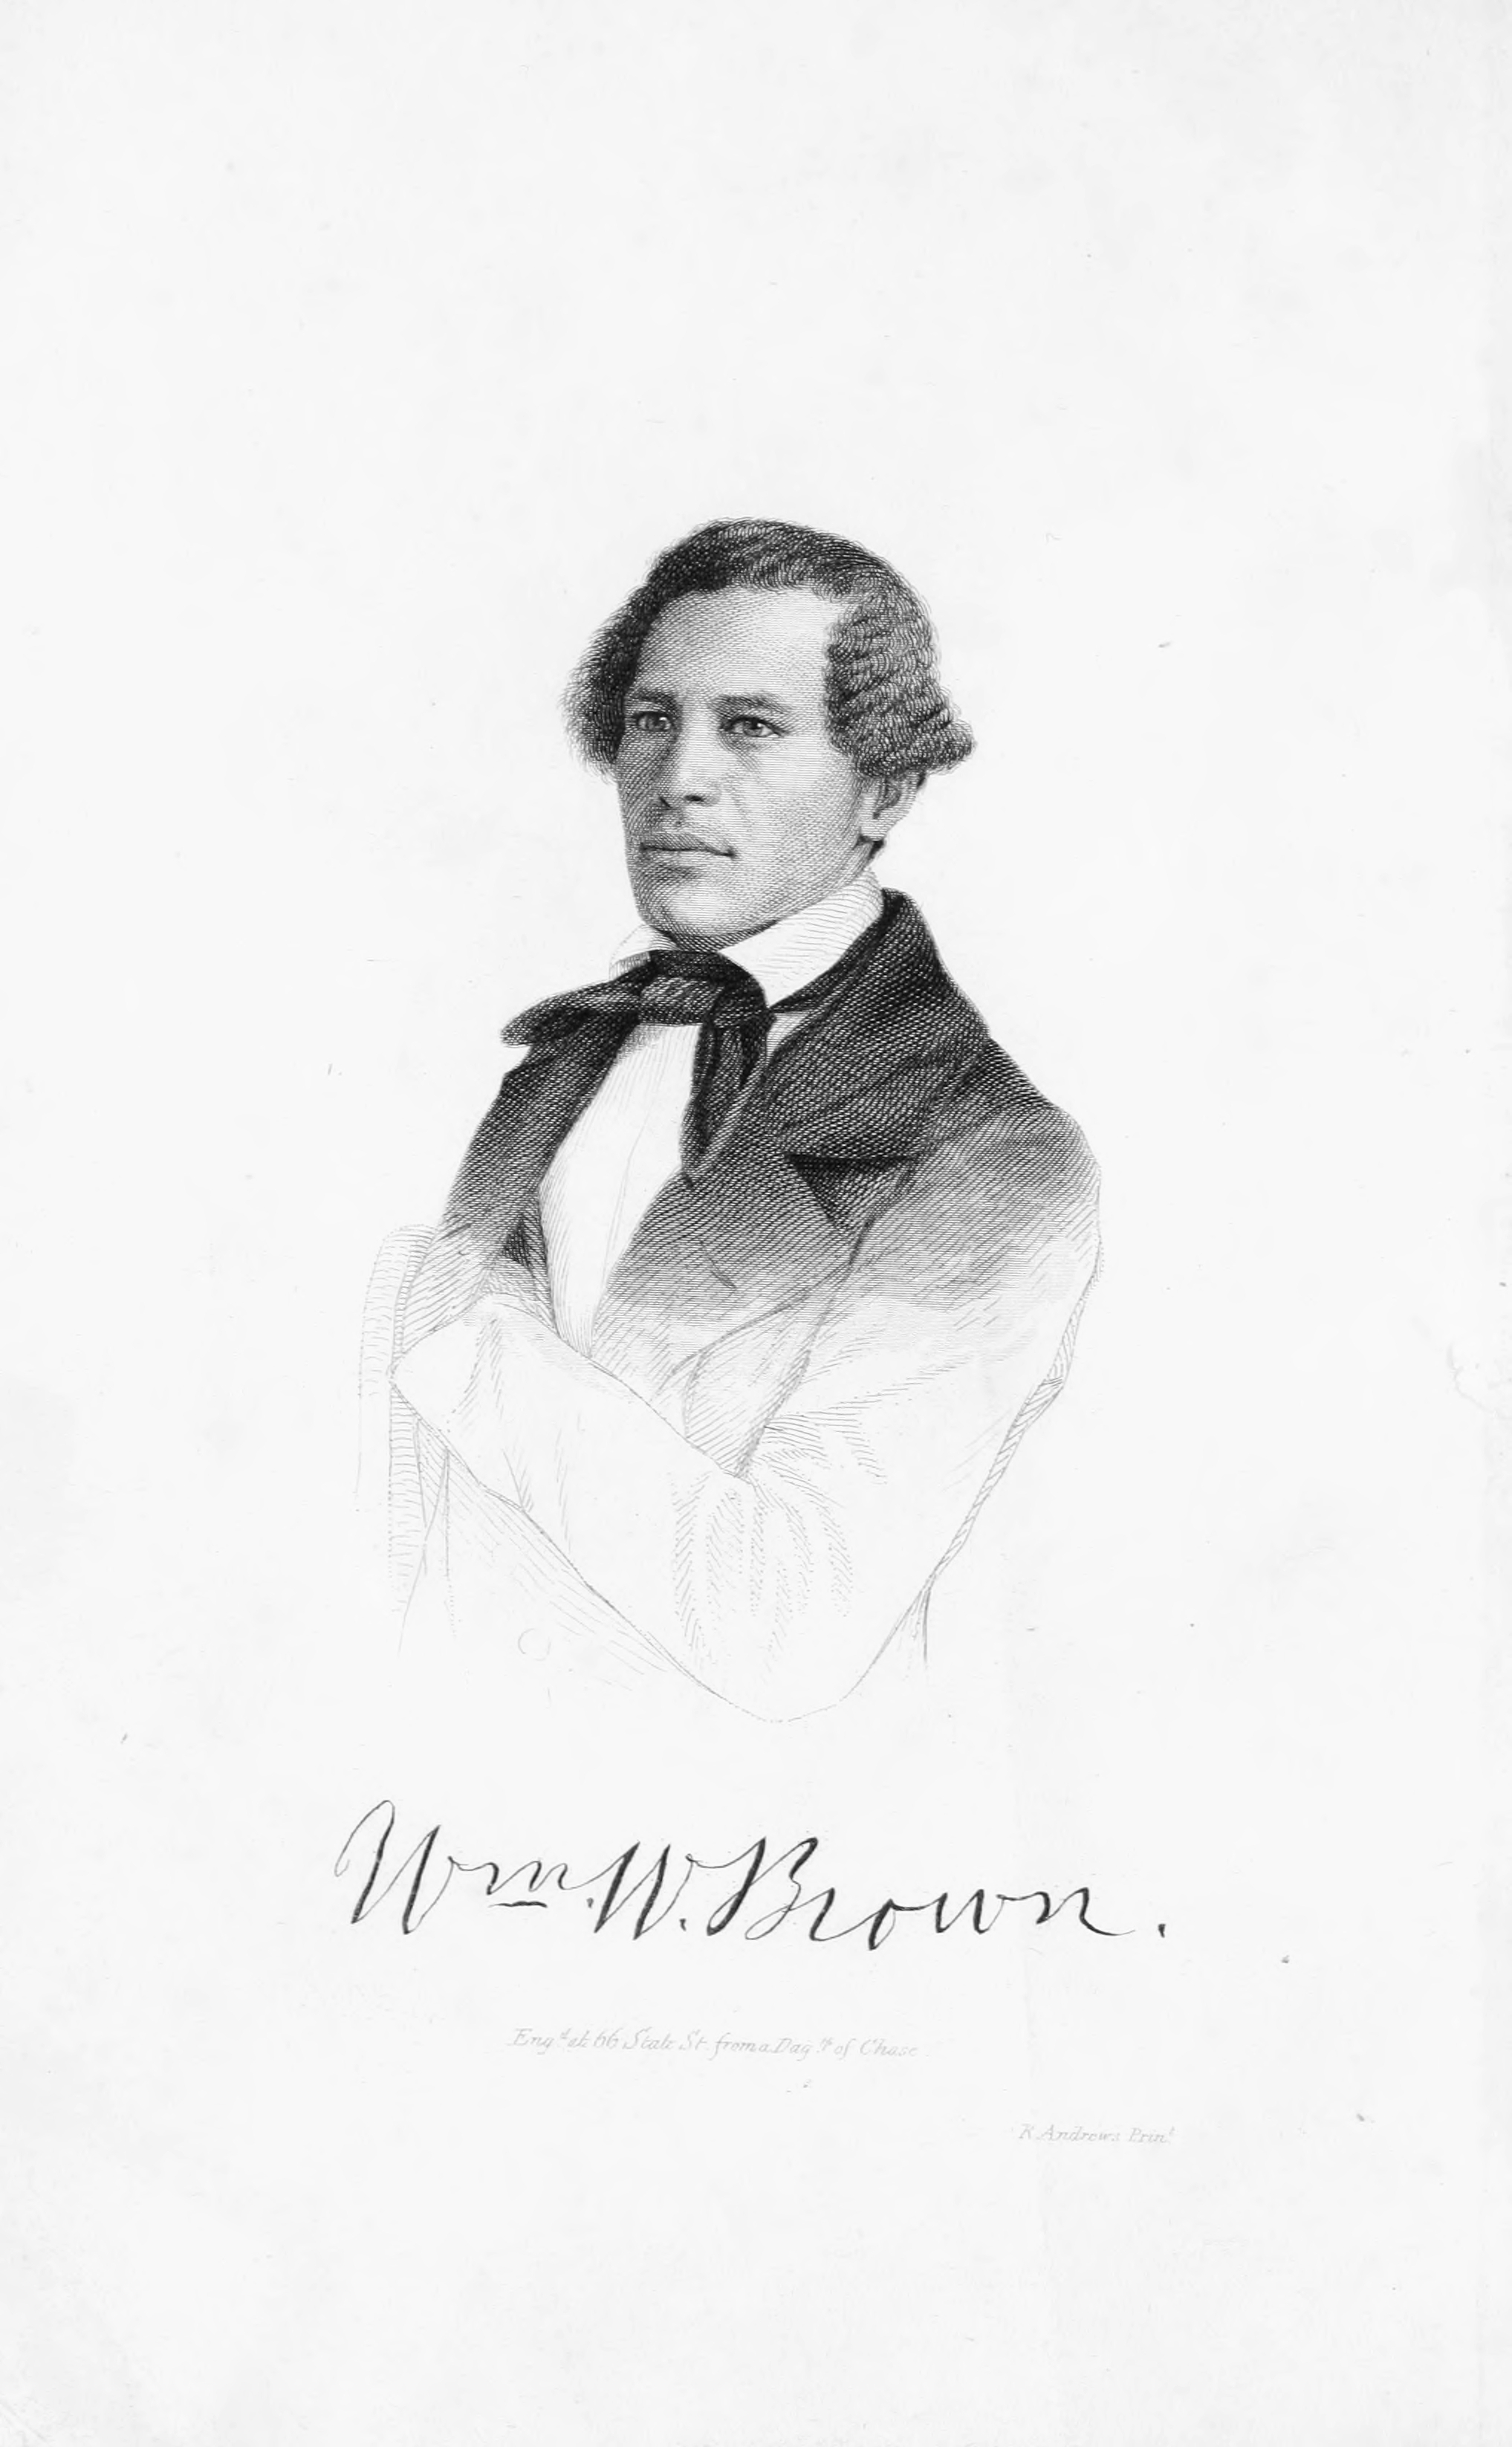
\includegraphics[width=134mm]{./imgs/front1.jpg}  \label{front}
  %\hfill
\end{adjustwidth}
  \caption{}
\end{figure}
\end{vplace}

\thispagestyle{empty}
\end{absolutelynopagebreak}


\pagebreak

\begin{absolutelynopagebreak}
\begin{vplace}
\begin{figure}[H]
\begin{adjustwidth}{-1.8cm}{}
  %\centering
  \vspace*{-2.6cm}
  %\hspace{-0.5cm}
  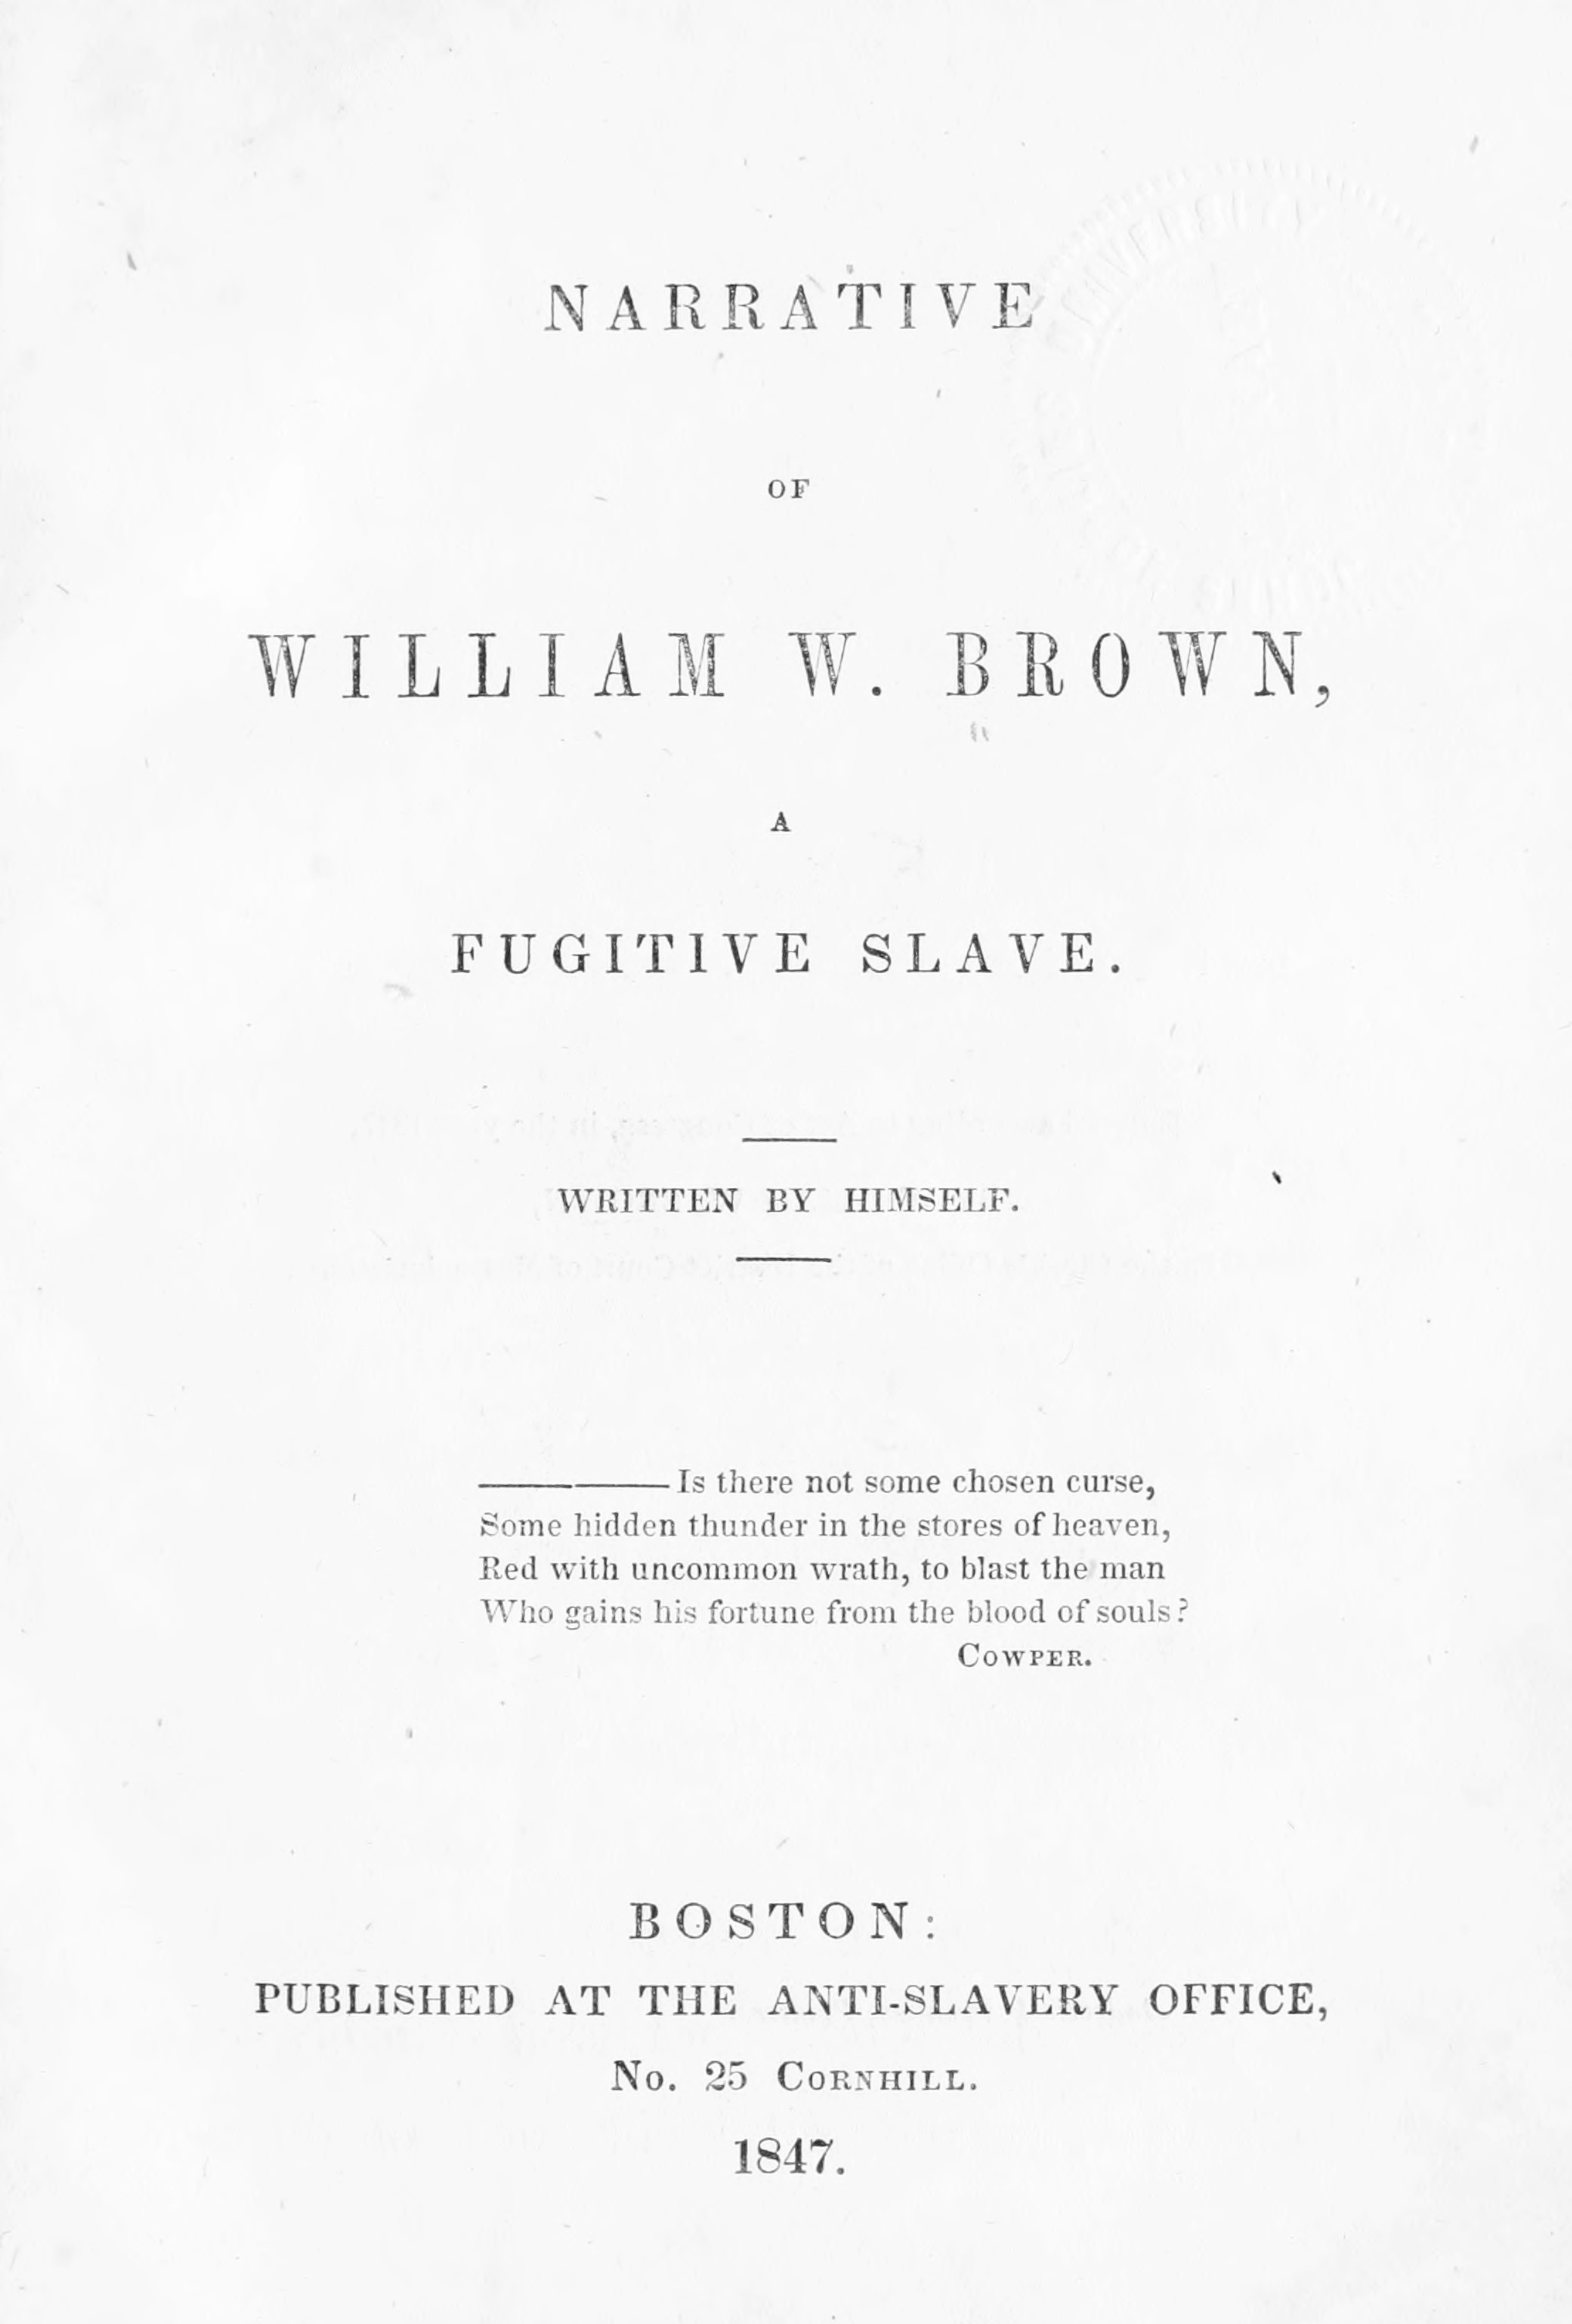
\includegraphics[width=134mm]{./imgs/front2.jpg}  
  %\hfill
\end{adjustwidth}
  \caption{Frontispício da primeira edição da autobiografia de William Wells Brown, publicada em Boston em 1847.}
\end{figure}
\end{vplace}

\thispagestyle{empty}
\end{absolutelynopagebreak}


\movetooddpage
\addcontentsline{toc}{part}{Narrativa de William Wells Brown}
\part*{Narrativa de William Wells Brown, escravo fugitivo, escrita por ele mesmo}


\chapter*{}
\thispagestyle{empty}
\begin{verse}
---Is there not some chosen curse,\\
Some hidden thunder in the stores of heaven,\\
Red with uncommon wrath, to blast the man\\
Who gains his fortune from the blood of \qb{}souls?\footnote{Tradução: ``Não haveria uma maldição seleta/ Um trovão oculto no arsenal celeste,/ Rubro com fúria especial, para fulminar o homem/ Que faz sua fortuna com o sangue das almas?''}
\end{verse}
\begin{flushright}
\versal{COWPER}\footnote{Brown atribui esses versos ao poeta inglês William
  Cowper (1731--1800). Na verdade, a passagem pertence à peça \emph{Cato,
  A Tragedy}, de Joseph Addison (1672--1719).}
\end{flushright}

\chapter{Para Wells Brown, de Ohio}

Treze anos atrás eu batia à sua porta, cansado, fugindo dos grilhões e
da chibata. Era forasteiro e você me hospedou. Estava faminto e você me
deu de comer. Estava nu e você me deu de vestir. A escravidão me negara
até um nome pelo qual pudesse ser chamado entre os homens, e você me deu
o seu. Eu seria uma criatura deveras vil se esquecesse tudo que te devo 
ou fizesse o que fosse para desonrar o seu nome sagrado!

Como pequeno testemunho da gratidão que tenho pelo meu primeiro
benfeitor, tomo a liberdade de lhe dedicar esta pequena \emph{Narrativa} dos
sofrimentos dos quais estava fugindo quando fui agraciado com a sua
compaixão. Entre as multidões que receberam seu auxílio, é bem possível
que você não se lembre de mim; mas até que eu esqueça Deus e a mim
mesmo, nunca me esquecerei de você.

Teu amigo agradecido

\begin{flushright}
\emph{William Wells Brown}
\end{flushright}

\chapter{Carta de Edmund Quincy} %, esq.

\begin{flushright}
\emph{Dedham, 1º de julho de 1847}
\end{flushright}

\begin{flushleft}
Para William Wells Brown
\end{flushleft}

Meu caro amigo: Agradeço sinceramente pelo privilégio de ler o
manuscrito da sua \emph{Narrativa}. Li"-a com profundo interesse e fiquei
emocionado. Tenho certeza que será, além de um enorme sucesso, de
extrema utilidade. Ela apresenta uma fase diferente do sistema
escravista infernal em relação àquela retratada na história admirável do
Sr.\,Douglass\footnote{Frederick Douglass (1819--1895): Abolicionista,
  jornalista e político americano. Sua primeira autobiografia, a
  \emph{Narrativa da vida de Frederick Douglass, um escravo americano},
  foi um sucesso de vendas na época e ainda é considerada um clássico da
  literatura dos \versal{EUA}.} e nos permite vislumbrar as crueldades atrozes de
outras partes do seu domínio.

As oportunidades que você teve de observar o funcionamento desse sistema
maldito foram particularmente grandes. Suas experiências na Lavoura, na
Casa Grande e, especialmente, no Rio, a serviço de Walker, o traficante
de escravos, quase não encontra paralelo entre outros indivíduos, e
certamente nenhum que tenha demonstrado a competência para descrevê"-los.
O que admiro, e o que me assombra, na sua \emph{Narrativa} é a calma e a
simplicidade com que descreve cenas e ações que poderiam muito bem
``levar as próprias pedras a se erguerem em motim'' contra a Instituição
Nacional que as tornam possíveis.

Como irá perceber, em muito pouco fiz uso da gentil permissão que me deu
para alterar aquilo que escreveras. Corrigir alguns equívocos, que \label{ref1}
pareciam ser meros erros de cópia, cometidos na pressa da composição,
empreendida em condições desfavoráveis, e sugerir alguns abreviamentos,
foi tudo que ousei fazer. Seria muita audácia da minha parte, e muita
vaidade também, tentar melhorar as descrições do que você viu e sofreu.
Algumas das cenas fariam jus ao próprio De Foe.

Confio que sua narrativa terá ampla circulação e tenho certeza de que
ela o merece. Deve possuir uma natureza diferente da minha o homem que
encerre a leitura da \emph{Narrativa} sem acreditar que entende a escravidão
melhor do que nunca, e a odeie ainda mais.

Fiel e respeitosamente, 

Seu amigo

\begin{flushright}
\emph{Edmund Quincy}
\end{flushright}

\chapter{Prefácio à primeira edição}

Os amigos da liberdade podem comemorar o surgimento da \emph{Narrativa} a
seguir, que acrescenta mais um volume à crescente literatura
antiescravista contemporânea. Como afirmou um grande observador da
natureza humana: ``Deixem"-me compor as canções de uma nação e não me
importarei com quem compõe suas leis'';\footnote{Frase de Andrew Fletcher
  (1655--1716), escritor e político antiunionista escocês.} e com o
mesmo grau de verdade pode"-se dizer que, entre um povo leitor como o
nosso, nossos livros irão ao menos caracterizar nossas leis. É uma
influência que avança silenciosamente em sua missão, mas jamais deixa de
encontrar o caminho a muitos corações calorosos para acender em seus
altares a chama da liberdade que um dia se conflagrará no incêndio que
há de consumir a opressão.

Este livreto é uma voz emanando da prisão, desvendando os feitos
sombrios que nela são perpetrados. Nossa causa recebe um grande socorro
dessa fonte. Os nomes daqueles que vieram de lá, e que batalharam
valorosamente pela justiça, não precisam ser registrados aqui. As obras
de alguns deles são monumentos eternos à divindade e seu registro
perpétuo encontra espaço nos corações agradecidos dos cativos redimidos.

Poucas pessoas tiveram maior oportunidade para conhecer a escravidão em
todos os seus aspectos mais terríveis do que William W. Brown. Ele
esteve por trás dos panos. Visitou suas câmaras secretas. Os ferros dela
penetraram a sua alma. Os laços mais caros da natureza foram fendidos em
sua pessoa. Uma mãe foi açoitada cruelmente perante seus próprios olhos.
Um pai\ldots{} mas, ah, escravo não tem pai. Um irmão se tornou vítima
de sua própria misericórdia. Uma irmã foi entregue ao controle
irresponsável do pálido opressor. E esta nação assente com a cena. A
União americana sanciona esses feitos. A Constituição protege os
criminosos. A religião americana santifica o crime. Mas a maré está
virando. Uma corrente submarina arrasta o país para a frente. Uma voz de
alerta, de admoestação, de censura, de rogo, está soando. Mãos seguram
mãos e corações se mesclam com corações na grande obra da salvação dos
escravos.

Mesmo agora, as convulsões do monstro evidenciam suas feridas profundas.

O autor desta \emph{Narrativa} foi emprestado pelo seu senhor para um
``\emph{traficante de almas}'' e testemunhou todos os horrores do
tráfico, desde a compra do rebanho humano nos estados criadores de
escravos, que produzem uma cena constante da separação das vítimas dos
seus entes queridos, até a sua venda final no mercado do Sul, para serem
exauridos em sete anos ou entregues à luxúria dos \emph{cristãos}
sulistas.

Muitas cenas pungentes são retratadas explicitamente, mas também com uma
simplicidade e uma engenhosidade que transmitem a certeza sobre a
veracidade da imagem.

Este livro fará muito para desmascarar aqueles que ``se vestiram com o
libré da corte celestial'' a fim de disfarçar a monstruosidade dos seus
atos.

Durante os últimos três anos, o autor dedicou todas as suas energias à
causa antiescravista. Labutando sob todas as deficiências e desvantagens
decorrentes de ter sido educado sob a escravidão, de ter sido sujeitado,
como foi desde nascença, a todos os males e privações inerentes à sua
condição, ainda assim ele seguiu em frente, atraído ao trabalho pelo
amor à liberdade, estimulado pela memória do próprio sofrimento, instado
pela consideração de que mãe, irmãos e irmã ainda agonizavam no
cativeiro ao lado de três milhões de filhos do Nosso Pai, sustentado por
uma fé inabalável na onipotência da verdade e no triunfo final da
justiça, para defender a causa dos escravos, e pela eloquência da sua
sinceridade transmitiu a certeza a muitas mentes e arregimentou a
simpatia e a cooperação de muitos outros em prol da causa.

Seu trabalho se limitou principalmente ao oeste do estado de Nova York,
onde conquistou muitos amigos queridos com seu zelo incansável, sua
energia perseverante, sua fidelidade constante e sua bondade universal.

Leitor, és um abolicionista? O que fizestes pelo escravo? O que fazes
por ele? O que pretendes fazer? Uma grande obra nos espera. Quem há de
ficar parado? Em termos comparativos, este é o grande movimento
humanitário da nossa era, engolindo, por ora, todas as outras questões.
O curso da história humana, obediente às leis imutáveis da nossa
existência, avança rapidamente para uma crise final. Eis a pergunta:

\begin{verse}
Have ye chosen, O my people, on whose \qb{}party ye shall stand,\\
Ere the Doom from its worn sandal shakes \qb{}the dust against our land?\footnote{Tradução: ``Já escolhestes, ó, meu povo, que partido ireis tomar,/ Antes que o Destino de suas sandálias gastas sacuda a poeira contra a
nossa terra?''. Versos de \emph{The Present Crisis}, do poeta
  romântico americano James Russell Lowell (1819--1891). ``Sacudir a
  poeira'' é uma referência a Mateus 10:14 e à antiga prática judaica de
  sacudir a poeira dos pés ao sair de cidades não"-judaicas para indicar
  separação do mundo gentio.}
\end{verse}

Você é cristão? Esta é a realização do Cristianismo prático, e não há
outra forma. O Cristianismo é \emph{prático} em sua própria essência e
natureza. É uma vida que nasce da alma imbuída com o seu espírito. É
amigo da causa missionária? Este é o maior empreendimento missionário de
hoje. Três milhões de \emph{cristãos}, transformados em pagãos pela lei,
anseiam pelas boas novas do Evangelho da liberdade. É amigo da Bíblia?
Vem, então, e nos ajuda a restaurar a vista para esses milhões cujos
olhos foram furados pela escravidão, para que possam enxergar e ler a
Bíblia. Ama Deus, a quem nunca viu? Então manifesta esse amor e devolve
ao irmão que já vistes a sua legítima herança, da qual foi privado por
tanto tempo e com tanta crueldade.

Não é por uma única geração de três milhões que trabalhamos, por mais
sublime que seja tal esforço. É pela humanidade, ao redor do mundo, não só agora, mas por todos os tempos, e por todas as gerações futuras:

\begin{verse}
For he who settles Freedom's principles,\\
Writes the death"-warrant of all tyranny.\footnote{Tradução: ``Pois quem estabelece os princípios da Liberdade/ Redige a sentença de morte
de toda a tirana.'' De \emph{L'Envoi}, poema final de \emph{A
  Year's Life}, o primeiro livro de James Russell Lowell.}
\end{verse}

É um trabalho vasto, um empreendimento glorioso, digno da devoção
inarredável de toda a vida dos grandes e dos bons.

O escravismo e os escravistas devem ser convertidos em seres
ignominiosos e detestáveis. Devem perder sua respeitabilidade e sua
reputação cristã. Devem ser tratados como ``ladrões de homens, culpados
do mais grave roubo e pecadores de primeira ordem''.\footnote{Passagem da
  Disciplina da Igreja Presbiteriana dos \versal{EUA}, adotada em 1794 e
  eliminada em 1816 com a influência crescente dos escravistas na
  Assembleia Geral.} Seus cúmplices mais culpados, na pessoa dos
\emph{apologistas nortistas}, tanto na Igreja quanto no Estado, devem
ser colocados na mesma categoria. Os homens honestos devem ser
convencidos a ver esses crimes com a mesma aversão e desprezo que
destinam aos ladrões e assassinos menos culpados, até que:


\begin{verse}
The common damned shun their society,\\
And look upon themselves as fiends less \qb{}foul.\footnote{Tradução: ``Os condenados comuns rejeitam a sua sociedade/ E se consideram demônios menos atrozes.'' De \emph{The Grave}, do poeta
  escocês Robert Blair (1699--1746).}
\end{verse}

Quando o crime da escravidão receber sua justa sentença, o trabalho
estará completo. E terá chegado o dia glorioso:

\begin{verse}
When man nor woman in all our wide \qb{}domain,\\
Shall buy, or sell, or hold, or be a slave.\footnote{Tradução: ``Quando nem homem nem mulher em nossos vastos domínios/ Há de comprar, ou vender, ou ter, ou ser escravo.'' Paráfrase dos versos finais de \emph{Inscription under the Picture of an Aged Negro"-woman}, do poeta escocês James Montgomery (1771--1854).}
\end{verse}

\bigskip

\begin{flushright}
\emph{J. C. Hathaway}

Farmington, Nova York, 1847.
\end{flushright}



\chapter*{Capítulo I}
\addcontentsline{toc}{chapter}{Capítulo \textsc{i}}

Nasci em Lexington, Kentucky. O homem que me roubou assim que nasci \label{ref5}
registrava o nascimento de todos os bebês que alegava serem de sua
propriedade em um livro que mantinha para esse fim. O nome de minha mãe
era Elizabeth. Ela teve sete filhos, a saber: Solomon, Leander,
Benjamin, Joseph, Millford, Elizabeth e eu. Nenhum de nós tinha o mesmo
pai que o outro. O nome de meu pai, como soube de minha mãe, era George
Higgins. Ele era um homem branco, aparentado com meu senhor, e ligado a
algumas das famílias mais proeminentes do Kentucky.

Meu senhor possuía cerca de quarenta escravos, vinte e cinco dos quais
eram lavradores. Ele se mudou do Kentucky para o Missouri quando eu era
ainda muito jovem e se estabeleceu cinquenta ou setenta quilômetros
acima de St.\,Charles, no Rio Missouri, onde, além da clínica de
medicina, praticava a moagem de cereais, o comércio e a agricultura. Ele
tinha uma fazenda grande, e seus principais produtos eram o tabaco e o
cânhamo. As senzalas ficavam situadas nos fundos da fazenda, com a casa
do feitor, chamado Grove Cook, em seu meio. Ele era encarregado de toda
a fazenda e, por não ter família, mantinha uma mulher que cuidava da
casa para ele; era ela a responsável por distribuir as provisões para os
lavradores.

Também havia uma mulher que ficava nos alojamentos para cozinhar para os
trabalhadores do eito, que eram convocados para a sua labuta incessante
todos os dias às quatro da manhã. O sino pendurado em um poste junto à
casa do feitor repicava e então eles tinham meia hora para fazer seu
desjejum e partir para o campo. Às quatro e meia, o feitor soava um
berrante, sinalizando o começo do trabalho, e todos que não estivessem
presentes naquele instante recebiam dez chibatadas do chicote com o qual
o feitor estava sempre armado. O cabo tinha quase um metro de
comprimento, com a ponta cheia de chumbo, e a chibata de couro tinha
dois metros, com arame trançado na ponta. O chicote era aplicado com
bastante frequência e liberdade, e qualquer pequeno delito por parte de
um escravo era causa para a sua utilização. Durante a época em que o Sr.\,Cook foi feitor, eu era criado doméstico, uma situação preferível à do
escravo do eito, pois eu era mais bem alimentado, me vestia melhor e não
era forçado a me levantar com o tocar do sino, e sim cerca de meia hora
depois. Muitas vezes fiquei deitado, escutando os estalos da chibata e
os berros dos escravos. Minha mãe trabalhava no eito e, uma manhã,
chegou ao campo dez ou quinze minutos depois dos outros. Logo que chegou
no local onde eles iriam trabalhar, o feitor começou a açoitá"-la.

--- Ah! por favor\ldots{} Ah! por favor\ldots{} Ah! por favor --- ela
gritava.

Essas eram as palavras recorrentes dos escravos, implorando por piedade
das mãos dos seus opressores. Eu reconheci a voz dela, saltei do meu
catre e saí correndo para a porta. A lavoura ficava longe da casa, mas
ainda assim eu escutava cada estalo do chicote, cada grito e gemido da
minha pobre mãe. Permaneci junto à porta, sem ousar ir além. Senti um
calafrio correr de cima a baixo e caí em prantos. Após a décima
chibatada, o som do chicote cessou e eu voltei para a cama, consolado
apenas pelas lágrimas. O sol ainda não havia nascido.

\chapter*{Capítulo II}
\addcontentsline{toc}{chapter}{Capítulo \textsc{ii}}

Meu senhor era um demagogo político e logo encontrou quem estivesse
disposto a obter"-lhe um cargo em troca dos favores que poderia prestar,
e poucos anos após sua chegada ao Missouri ele foi eleito para o
Legislativo estadual. Enquanto ele estava ausente, o Sr.\,Cook, o feitor,
ficava encarregado de tudo, e logo se tornou ainda mais tirânico e
cruel. Entre os escravos da fazenda havia um que atendia pelo nome de
Randall. Era um homem de cerca de um metro e oitenta de altura, esbelto,
conhecido por todos por sua enorme força, e considerado o escravo mais
valioso e capaz de toda a plantação; contudo, por melhor ou mais útil
que seja um escravo, ele quase nunca escapa da chibata. Mas Randall era
uma exceção. Ele estava na fazenda desde que eu me lembrava, mas eu
nunca o vira ser castigado. Isso não era graças ao senhor ou ao feitor.
Muitas vezes eu o ouvi declarar que nenhum branco jamais o açoitaria,
que morreria antes disso.

Desde o dia em que chegara à fazenda, Cook sempre declarara que podia e
iria castigar qualquer crioulo que trabalhasse sob o seu comando no
campo. Meu senhor lhe dissera inúmeras vezes que não tentasse açoitar
Randall, mas o feitor estava decidido. Assim que se tornou o único
ditador da fazenda, determinou que chegara o momento de executar suas
ameaças. Um dia, ordenou uma tarefa muito difícil, mais do que Randall
seria capaz de fazer; e à noite, como a tarefa não estava concluída,
disse a Randall que deveria lembrar dele na manhã seguinte. No outro
dia, depois que os escravos haviam feito seu desjejum, Cook chamou
Randall e disse que pretendia açoitá"-lo. O feitor ordenou que ele
cruzasse as mãos e fosse amarrado. Randall perguntou por que queria
açoitá"-lo. A resposta foi que ele não completara a tarefa do dia
anterior. Randall disse que a tarefa era grande demais, e que a teria
realizado se não fosse por isso. Cook respondeu que não fazia diferença,
que era preciso açoitá"-lo. Randall ficou em silêncio por um instante e
então respondeu:

--- Sr.\,Cook, eu sempre tentei agradá"-lo desde que o senhor chegou à
fazenda, mas o senhor está decidido a não se satisfazer com o meu
trabalho. Deixe"-me trabalhar como posso. Homem nenhum colocou as mãos em
mim para me açoitar nos últimos dez anos, e há muito concluí que não
existe homem vivo que vá me açoitar.

Cook, percebendo pelo olhar e os gestos decididos de Randall que este
iria resistir, chamou três escravos que estavam trabalhando, ordenou
que agarrassem Randall e o amarrassem. Os escravos ficaram parados; eles
conheciam Randall, e sabiam muito bem a força deste, então tinham medo
de atacá"-lo. Logo que Cook ordenou que os homens o agarrassem, Randall
se virou para eles e disse:

--- Rapazes, vocês todos me conhecem, sabem que posso com qualquer de
vocês três e que o homem que encostar em mim há de morrer. Esse branco
não consegue me castigar sozinho, então chamou vocês para ajudá"-lo.

O feitor não conseguiu convencê"-los a amarrar Randall e finalmente
ordenou que todos voltassem para o trabalho.

Randall não ouviu nada do feitor por mais de uma semana. Uma manhã, no
entanto, enquanto os escravos estavam no eito, ele chegou com três
amigos, Thompson, Woodbridge e Jones. Eles foram até onde Randall estava
trabalhando e Cook ordenou que deixasse o trabalho de lado e os
acompanhasse até o celeiro. Randall se recusou, então foi atacado pelo
feitor e seus companheiros; ele reagiu e os derrotou um a um,
prostrando"-os no chão. Woodbridge sacou sua pistola e disparou,
derrubando"-o com uma bala. Os outros saltaram sobre ele, desferindo
porretadas sobre a cabeça e no rosto até que conseguiram amarrá"-lo.
Depois, Randall foi levado ao celeiro e amarrado a uma trave. Cook lhe
deu mais de cem chibatadas com um chicote de couro pesado, mandou lavar
as feridas com salmoura e deixou"-o amarrado durante o dia. No dia
seguinte, ele foi desamarrado e levado à ferraria, onde uma bola com
corrente foi presa à sua perna. Randall foi forçado a trabalhar no campo
e completar a mesma quantidade de trabalho que todos os outros. Quando
voltou para casa, seu senhor ficou muito contente em descobrir que
Randall fora domado na sua ausência.

\chapter*{Capítulo III}
\addcontentsline{toc}{chapter}{Capítulo \textsc{iii}}

Pouco depois, meu senhor se mudou para a cidade de St.\,Louis e comprou
uma fazenda a seis quilômetros de distância, que colocou sob a
supervisão de um feitor chamado Friend Haskell, um típico yankee da Nova
Inglaterra. Os yankees são famosos por darem os feitores mais cruéis de
todos.

Minha mãe foi alugada na cidade, e eu também fui alugado lá pelo Major
Freeland, que mantinha uma taverna. Oriundo da Virgínia, ele estava
envolvido com corridas de cavalo, rinhas de galos e jogos de azar e era
um bêbado inveterado. Havia dez ou doze criados na casa e, quando ele
estava presente, o lugar era uma balbúrdia e um pandemônio. Em seus
acessos de fúria, ele atirava cadeiras nos criados; em seus momentos
mais racionais, quando desejava castigar alguém, os amarrava e açoitava
no defumadouro, então acendia uma fogueira com talos de tabaco para
defumá"-los. Isso que ele chamava de uma ``\emph{virginiada}''.

Reclamei para o meu senhor do tratamento que recebia do Major Freeland,
mas não fez diferença. Ele não dava nenhuma importância a isso, desde
que recebesse o dinheiro pelo meu trabalho. Após morar com o Major \enlargethispage{\baselineskip}
Freeland por cinco ou seis meses, fugi e me escondi na floresta perto da
cidade. Quando a noite caiu, me dirigi à fazenda do meu senhor, mas tive
medo de ser avistado, sabendo que se o feitor, o Sr.\,Haskell, me
achasse, eu seria arrastado de volta para o Major Freeland; assim,
permaneci na floresta. Um dia, enquanto estava na floresta, ouvi cães
ladrando e uivando, e logo eles se aproximaram tanto que reconheci os
sabujos do Major Benjamin O'Fallon, que criava cinco ou seis cães para
caçar escravos fugitivos.

Logo que me convenci de que eram eles, soube que a fuga seria
impossível. Encontrei refúgio na copa de uma árvore e os cães logo a
cercaram, e ali permaneceram até os caçadores chegarem, meia hora ou
três quartos de hora depois. Dois homens acompanhavam os cães e, assim
que chegaram, me mandaram descer. Eu desci e fui amarrado e levado à
cadeia de St.\,Louis. O Major Freeland logo apareceu, me soltou e ordenou
que eu o seguisse, o que fiz. Após voltarmos para casa, ele me amarrou
no defumadouro e eu fui açoitado horrivelmente. Após o Major me castigar
até se dar por satisfeito, ele mandou chamar Robert, seu filho, um jovem
de dezoito ou vinte anos, para garantir que eu fosse defumado. Ele
acendeu uma fogueira com talos de tabaco que logo me deixou tossindo e
espirrando. Esse era o modo como seu pai lidava com seus escravos na
Virgínia, Robert me contou. Após aplicarem o que consideravam uma
defumada decente, fui desamarrado e colocado no trabalho mais uma vez.

Robert Freeland era ``filho de peixe''. Apesar de muito jovem,
frequentemente chegava em casa embriagado. Creio que hoje ele é o
comandante popular de um barco a vapor no rio Mississippi. Os negócios
do Major Freeland logo decaíram e eu fui colocado a bordo do vapor
\emph{Missouri}, que fazia a rota entre St.\,Louis e Galena. O comandante
do navio era William B. Culver. Permaneci a bordo durante a temporada de
navegação, a época mais agradável que havia vivenciado até então. Ao
final do período, fui alugado pelo Sr.\,John Colburn, que mantinha o
Missouri Hotel. Ele era oriundo de um dos Estados Livres, mas não acho
que jamais pôs os pés nesta terra de Deus um inimigo mais inveterado dos
negros. Na época, o hotel era um dos maiores da cidade e empregava vinte
ou trinta criados, quase todos escravos.

O Sr.\,Colburn era muito perverso, e não apenas com os criados, mas com a
esposa também, uma excelente mulher e uma pessoa da qual nunca observei
um criado receber uma única palavra de rispidez, assim como nunca
observei uma palavra de gentileza do marido. Entre os escravos
empregados no hotel havia um chamado Aaron, que pertencia ao Sr.\,John F.
Darby, um advogado. Aaron lavava as facas. Um dia, uma das facas foi
colocada à mesa menos limpa do que poderia estar. Por essa ofensa, o Sr.\,Colburn atou Aaron no depósito de lenha e lhe deu cinquenta chibatadas
nas costas nuas com um chicote de couro, e depois me fez lavar Aaron com
rum. Isso pareceu deixá"-lo em mais agonia do que as vergastadas. Depois
que foi desamarrado, ele voltou para a casa do seu senhor e reclamou do
tratamento que recebera. O Sr.\,Darby também não deu nenhuma atenção ao
que ele tinha a dizer e o mandou de volta na mesma hora. Colburn, ao
descobrir que Aaron fora reclamar para o seu senhor, o amarrou de novo e
o castigou pior do que antes. As costas do pobre rapaz foram
literalmente cortadas em pedacinhos, tanto que não teve como trabalhar
pelos próximos dez ou doze dias.

Entre os criados havia também uma menina de nome Patsey cujo senhor
morava no campo. Uma noite, o Sr.\,Colburn a amarrou e açoitou até que
vários dos hóspedes apareceram para implorar que ele parasse. O motivo
para o castigo era o seguinte. Ela estava noiva de um homem que
pertencia ao Major William Christy, que residia seis ou sete quilômetros
ao norte da cidade. O Sr.\,Colburn a proibira de ver John Christy.
Supostamente, o motivo era o apreço que ele mesmo tinha por Patsey. Ela
foi encontrá"-lo naquela tarde e John voltou para casa com ela. O Sr.\,Colburn pretendia castigar John se ele passasse pelo cercado, mas este
conhecia muito bem o temperamento do rival e se manteve a uma distância
segura. Assim, ele extraiu sua vingança da pobrezinha. Se todos os
capatazes do mundo fossem reunidos, não creio que se encontraria entre
eles um homem mais cruel do que John Colburn, e este um nortista ainda
por cima.

Enquanto eu morava no Missouri Hotel, ocorreu uma circunstância que me
causou enorme infelicidade. Meu senhor vendeu minha mãe e todos os seus
filhos, exceto por mim. Foram todos vendidos para pessoas diferentes na  
cidade de St.\,Louis.

\chapter*{Capítulo IV}
\addcontentsline{toc}{chapter}{Capítulo \textsc{iv}}

Logo fui retirado das mãos do Sr.\,Colburn e alugado para Elijah P.
Lovejoy, na época editor e proprietário do \emph{St.\,Louis Times}. Nesse
período, meu trabalho era principalmente na tipografia, atendendo os
trabalhadores, manejando a prensa etc. O Sr.\,Lovejoy era um homem muito
bom, absolutamente o melhor senhor que jamais tive. A ele mais do que
ninguém, e ao meu emprego na tipografia, devo o pouco aprendizado que
obtive na escravidão.

Apesar de haver quem considerasse que a escravidão era leve no Missouri,
em comparação com os estados onde se cultiva algodão, açúcar e arroz,
não há parte do nosso país escravista mais famoso pelo barbarismo dos
seus habitantes do que St.\,Louis. Foi aqui que o Coronel Harney, oficial
dos Estados Unidos, açoitou uma escrava até a morte. Foi aqui que
Francis McIntosh, um negro livre de Pittsburgh, foi arrancado do vapor
\emph{Flora} e queimado na fogueira. Durante meus oito anos de
residência na cidade, pude observar pessoalmente inúmeros casos de
extrema crueldade; registrar todos eles ocuparia mais espaço do que
jamais seria possível neste pequeno volume. Assim, apresentarei apenas
mais alguns, além daqueles que já relatei.

O Capitão J. B. Brunt, que residia próximo ao meu senhor, tinha um
escravo chamado John. Este era seu criado pessoal, cocheiro etc. Em uma
ocasião, enquanto guiava seu senhor pela cidade, estando as ruas muito
lamacentas e os cavalos galopando à velocidade, um pouco de lama
respingou em um cavalheiro chamado Robert More. More estava decidido a
se vingar. Três ou quatro meses após o ocorrido, ele comprou John com o
objetivo expresso, disse ele, de ``domar esse mal***o crioulo''. Após a
compra, ele o levou a um ferreiro, prendeu bola e corrente à sua perna e
o colocou a guiar uma parelha de bois. John ficou preso no trabalho
árduo até o ferro ao redor da sua perna desgastar tanto a carne que a
mortificação parecia garantida. Além disso, John me contou que seu
senhor o açoitou regularmente três vezes por semana pelos dois primeiros
meses, e tudo isso para ``domá"-lo''. Seria impossível encontrar em toda
St.\,Louis um homem de aspecto mais nobre do que John antes de cair nas
mãos de More; e uma criatura mais degradada e de espírito mais subjugado
não se encontraria em qualquer fazenda sulista após ele ter sido
sujeitado a esse processo de ``domação'' por três meses. Na última vez
que o vi, ele havia perdido quase completamente o uso dos membros.

Enquanto morava com o Sr.\,Lovejoy, eu frequentemente era mandado aos
escritórios do \emph{Missouri Republican}, publicado pelo Sr.\,Edward
Charles, para fazer pequenas tarefas. Uma vez, enquanto voltava para o
escritório carregando tipos, fui acossado por vários meninos maiores,
filhos de escravistas, que me atacaram com bolas de neve. Por estar
carregando os tipos pesados nas mãos, eu não podia correr deles, então
coloquei os tipos no chão e reagi. Eles se reuniram ao meu redor,
atirando pedras e pedaços de pau até me dominarem, e teriam me capturado
se eu não tivesse saído em disparada. Com a minha retirada, eles se
apossaram dos tipos, e eu não conseguia imaginar como recuperá"-los.
Sabendo que o Sr.\,Lovejoy era um homem muito benevolente, voltei para o
escritório e expliquei para ele toda a situação. Ele me mandou
permanecer onde estava, recrutou um dos aprendizes e foi atrás dos
tipos. Ele logo retornou com o material, mas na volta me informou que
Samuel McKinney lhe dissera que pretendia me açoitar, pois eu havia
machucado seu filho. Logo depois, um dos tipógrafos avistou McKinney se
dirigindo ao escritório e me avisou, permitindo que eu fugisse pela
porta dos fundos.

Como eu não estava lá quando chegou no escritório, McKinney saiu
enfurecido, jurando que me açoitaria até a morte. Alguns dias depois,
enquanto eu caminhava pela Rua Principal, ele me agarrou pela gola e me
deu cinco ou seis bengaladas violentas na cabeça, fazendo com que o
sangue jorrasse do meu nariz e das minhas orelhas de tal forma que
minhas roupas ficaram completamente saturadas de sangue. Após me
espancar o quanto quis, ele me soltou. Eu voltei para o escritório tão
enfraquecido com a perda de sangue que o Sr.\,Lovejoy me mandou para
casa, de volta para o meu senhor. Cinco semanas se passaram antes que eu
voltasse a caminhar. Durante esse período, foi necessário que alguém me
substituísse no escritório, então perdi meu emprego.

Depois que me recuperei, fui alugado pelo Capitão Otis Reynolds como
camareiro de bordo do vapor \emph{Enterprize}, de propriedade dos
senhores John e Edward Walsh, agentes comerciais de St.\,Louis. Na época,
o navio trafegava no Alto Mississippi. Minha função a bordo era atender
cavalheiros e, como o capitão era um bom homem, a posição me agradava;
mas ao estar sempre de um lugar para outro, vendo rostos novos todos os
dias, e sabendo que eles podiam ir aonde bem entendessem, logo fiquei
infeliz. Várias vezes, pensei em desembarcar em algum lugar e tentar uma
fuga para o Canadá, onde sempre ouvira falar que os escravos podiam
viver, ser livres e ficar protegidos.

Mas sempre que essas ideias me ocorriam, minha determinação logo era
abalada pela memória de minha cara mãe, ainda escrava em St.\,Louis, e eu
não suportava a ideia de deixá"-la naquela situação. Tantas vezes ela me
sentara no joelho e contara como me carregara nas costas quando eu era
bebê enquanto trabalhava no eito, chegando a ser frequentemente
castigada por deixar o trabalho para me amamentar, como eu parecia feliz
quando ela me pegava no colo. Quando lembrava disso, decidia nunca
abandonar a terra da escravidão sem minha mãe. Eu pensava que deixá"-la
na escravidão, após tudo o que ela passara e sofrera por mim, seria
renegar tudo o que devia a ela. Além disso, eu tinha três irmãos e uma
irmã na cidade (dois dos meus irmãos haviam morrido).

Minha mãe, meus irmãos Joseph e Millford e minha irmã Elizabeth
pertenciam ao Sr.\,Isaac Mansfield, oriundo de um dos Estados Livres
(Massachusetts, creio). Funileiro por profissão, ele comandava uma
grande manufatura. De todos os meus parentes, minha mãe era a primeira,
minha irmã a segunda. Uma tarde, enquanto as visitava, fiz alguma alusão
à minha proposta de viajar para o Canadá. Minha irmã se sentou ao meu
lado, tomou minhas mãos nas suas e, com os olhos cheios de lágrimas,
disse:

--- Meu irmão, você não vai abandonar mamãe aqui, e sua querida irmã
também, sem um amigo sequer no mundo, vai?

Eu olhei no seu rosto banhado em lágrimas e caí em prantos também.

--- Não, eu nunca hei de desertar você e mamãe.

Ela apertou minhas mãos e disse:

--- Meu irmão, você sempre declara que não vai terminar seus dias na
escravidão. Não consigo imaginar nenhum jeito possível de escapar
conosco; e agora, irmão, você está em um barco a vapor, onde tem alguma chance
de fugir para a terra da liberdade. Por favor, não se prenda por nós. Se
não pudermos obter a nossa liberdade, não queremos ser nós o motivo para
impedi"-lo de conquistar a sua.

Eu não conseguia mais conter meus sentimentos, e quando os extravasei
ela deixou de tocar no assunto. Contrário aos desejos delas, jurei para
mim mesmo que não as deixaria nas mãos do opressor. Parti de volta para
o navio e deitei no meu catre, mas ``o sono fugiu dos meus olhos e o
repouso das minhas pálpebras''.

Algumas semanas depois, na nossa passagem para o Sul, uma turma de
escravos embarcou em Hannibal, com destino ao mercado em Nova Orleans. A
turma era composta por cinquenta ou sessenta homens e mulheres de dezoito a 
quarenta anos. Uma turma de escravos em um navio a vapor sulista, indo
em direção às regiões do algodão e do açúcar, é uma ocorrência tão comum
que ninguém, nem mesmo os passageiros, parecia notar, apesar das
correntes retinirem com cada passo que davam. Contudo, havia um membro
dessa turma que chamava a atenção dos passageiros e da tripulação. Era
uma linda menina, aparentando vinte anos de idade, perfeitamente branca,
com cabelo claro e liso e olhos azuis. Mas não era a brancura da sua
pele que causava sensação em quem a avistava, era sua beleza
praticamente ímpar. A bordo, não demorou para que atraísse os olhos de
todos os passageiros, incluindo as damas, e que o assunto de todas as
conversas fosse a linda escrava. Ela não estava acorrentada. O homem que
reclamava para si esse artigo de mercadoria humana era um tal Sr.\,Walker, um famoso traficante de escravos que residia em St.\,Louis. Entre
passageiros e tripulação, havia uma ânsia geral pela história da menina.
Seu senhor a mantinha sempre junto de si, e teria sido considerado
impudente da parte dos passageiros se dirigir a ela, enquanto os
tripulantes ficavam proibidos de conversar com eles o mínimo que fosse.
Quando chegamos a St.\,Louis, os escravos foram transferidos para um
barco com destino a Nova Orleans, então o histórico dessa bela escrava
permaneceu um mistério.

Continuei a bordo durante a temporada, e não raro tínhamos no navio
turmas de escravo a caminho das fazendas de algodão, açúcar e arroz do
Sul.

Na segunda metade do verão, o Capitão Reynolds deixou o barco e eu fui
mandado para casa. A seguir, fui mandado para trabalhar na fazenda sob o
Sr.\,Haskell, o feitor. Como eu estava longe do campo havia algum tempo,
e desacostumado a trabalhar sob o sol escaldante, foi muito difícil, mas
fui forçado a acompanhar o ritmo dos melhores escravos.

Descobri que havia uma enorme diferença entre o trabalho na cabine de um
navio a vapor e o trabalho em um milharal.

Meu senhor, que estava morando na cidade, logo se mudou para a fazenda,
então eu fui retirado do campo e levado para trabalhar de atendente na
casa grande. Sua esposa era rabugenta e difícil de agradar, mas eu muito
preferia estar sob o seu controle do que do feitor. Eles levaram consigo
o Sr.\,Sloane, um ministro presbiteriano; a Srta.\,Martha Tulley, sua
sobrinha do Kentucky; e William, seu sobrinho. O último frequentava a
família havia vários anos, mas os outros eram recém"-chegados.

O Sr.\,Sloane era um ministro jovem, estava no Sul havia muito pouco
tempo e parecia que todo o seu objetivo de vida era agradar os
escravistas, especialmente meu senhor e minha senhora. Ele pretendia
visitá"-los durante o inverno e não só tentou agradá"-los, creio que foi
admiravelmente bem"-sucedido. Quando eles queriam música, ele cantava;
quando queriam orações, rezava; quando queriam uma história, contava. Em
vez de ensinar teologia ao meu senhor, meu senhor ensinou teologia a
ele. Enquanto estava com o Capitão Reynolds, meu senhor havia
``descoberto a religião'', então havia novas leis na fazenda. Antes, aos
domingos, tínhamos o privilégio de caçar, pescar, fabricar vassouras e
cestos etc., mas tudo isso parou. Agora, todos os domingos éramos
forçados a participar de cultos. Nosso senhor era tão religioso que
convenceu outros a se juntar a ele para contratar um pastor a fim de
pregar para os escravos.

\chapter*{Capítulo V}
\addcontentsline{toc}{chapter}{Capítulo \textsc{v}}

Meu senhor fazia a família orar de manhã e à noite. À noite, os escravos
eram chamados para participar; pelas manhãs, no entanto, eles precisavam
estar no trabalho, então o senhor cuidava de todas as orações. Meu
senhor e minha senhora eram grandes entusiastas do \emph{mint
julep},\footnote{Coquetel tradicional do sul dos \versal{EUA} à base de bourbon,
  hortelã, xarope e gelo triturado.} e todas as manhãs se preparava uma
jarra cheia, da qual eles bebiam livremente, incluindo o jovem William.
Depois que todos bebiam com gosto, eles faziam as orações da família e
então o desjejum. Não posso negar que amava o \emph{julep} tanto quanto
eles, e durante as orações sempre tomava cuidado para me sentar perto da
mesa onde a jarra ficava para me servir enquanto eles se ocupavam das
suas devoções. Quando eles terminavam de rezar, ninguém estava mais
feliz do que eu. Uma manhã, ocorreu um acidente triste. Enquanto me
servia e ficava de olho na minha velha senhora ao mesmo tempo,
acidentalmente deixei a jarra cair no chão, que se despedaçou toda, e
derramou a bebida. Foi um mau bocado para mim; assim que as orações
terminaram, fui levado e castigado duramente.

A família do meu senhor era constituída por ele, pela esposa e pelo
sobrinho, William More, que fora adotado quando tinha poucas semanas.
Como ele e eu tínhamos o mesmo nome, o meu foi alterado para dar
precedência ao dele, apesar de eu ser dez ou doze anos mais velho. Como
a fazenda ficava a seis quilômetros da cidade, eu precisava guiar a
família até a igreja. Eu sempre odiava a chegada do domingo, pois,
durante o culto, era forçado a ficar junto aos cavalos, sob o sol
escaldante ou então na chuva, dependendo do dia.

Um domingo, enquanto passávamos pela casa de D.\,D.\,Page, um cavalheiro
proprietário de uma grande padaria, eu estava sentado na boleia, que
ficava bastante elevada, quando vi o Sr.\,Page perseguindo um escravo
pelo jardim, estalando um chicote comprido e acertando"-o com cada salto.
O homem logo fugiu do quintal, seguido pelo Sr.\,Page. Eles passaram
correndo por nós e, quando o escravo percebeu que seria alcançado, parou
de repente. Page tropeçou nele e caiu nas pedras da calçada, quebrando
uma das pernas e ficando aleijado pelo resto da vida. O mesmo
cavalheiro, pouco tempo antes, havia amarrado Delphia, uma de suas
mulheres, e a açoitado quase até a morte; contudo, ele era também
diácono da igreja batista e em boa situação com todos. Pobre Delphia! Eu
a conhecia bem e fui chamado para visitá"-la na sua convalescença; nunca
hei de me esquecer do seu estado. Ela pertencia à mesma igreja que o seu
senhor.

Logo depois disso, fui alugado pelo Sr.\,Walker, o mesmo homem que
mencionei que carregava turmas de escravos rio abaixo no vapor
\emph{Enterprize}. Ao me encontrar no posto de camareiro de bordo, e
acreditando que eu seria a pessoa certa para cuidar dos escravos, ele
decidiu me empregar para esse propósito; quando descobriu que meu senhor
não estava disposto a me vender, ele me alugou pelo período de um ano.

Quando descobri que fora alugado para um especulador de negros, ou
``traficante de almas'', como os escravos costumavam chamá"-los, ninguém
seria capaz de imaginar minha emoção. O Sr.\,Walker oferecera um preço
alto por mim, como viria a descobrir, mas imagino que meu senhor não
podia me vender, pois eu e ele éramos parentes próximos. Quando fui
trabalhar para o Sr.\,Walker, descobri que minha chance de fugir para a
terra da liberdade passara, pelo menos por ora. Ele tinha uma turma de
escravos pronta para Nova Orleans, e em poucos dias nossa jornada
começou. Não tenho palavras para expressar meus sentimentos naquela \label{ref6}
ocasião. Apesar do meu senhor ter dito que não havia me vendido, e o Sr.\,Walker ter dito que não me comprara, eu não acreditava neles; foi só
após visitar Nova Orleans e estar a caminho de volta que acreditei que
não havia sido vendido.

O navio tinha um salão grande no convés inferior onde os escravos eram
mantidos, homens e mulheres, promiscuamente. Eles ficavam acorrentados
aos pares, sob vigilância constante para garantir que não se soltassem;
já ocorreram casos de escravos soltarem suas correntes e fugirem nos
desembarcadouros, quando os navios param para carregar madeira. Apesar
de todo o nosso cuidado, perdemos uma mulher que havia sido tirada do
marido e dos filhos; como não desejava viver sem eles, com a alma
agonizando, ela saltou pela borda fora e se afogou. Ela não estava
acorrentada.

Era quase impossível manter aquela parte do barco limpa.

Ao atracar em Natchez, os escravos foram todos levados para o
barracão,\footnote{No original, \emph{slave"-pen}. Termo usado na literatura
  antiescravista para referir"-se ao edifício que servia de loja para a
  venda dos escravizados, mas que também possuía elementos de prisão (grades
  e algemas) para o confinamento dos cativos.} onde foram mantidos por
uma semana, durante a qual vários foram vendidos. O Sr.\,Walker
alimentava bem seus escravos. Em St.\,Louis, carregamos várias centenas
de quilos de toicinho defumado e farinha de milho, e seus escravos se
alimentavam melhor do que o normal em Natchez, até onde pude observar.

Ao final da semana, partimos para Nova Orleans, nosso destino final,
onde chegamos após dois dias. Lá, os escravos foram colocados em um
barracão, onde aqueles que desejavam comprá"-los podiam examiná"-los. O
barracão era um pátio pequeno, cercado de edifícios, de cinco a sete
metros de largura, com exceção de um portão com grades de ferro. Os
escravos eram mantidos nos edifícios durante a noite e mandados para o
pátio durante o dia. Depois que os melhores eram negociados em vendas
privadas no barracão, o resto era levado ao Exchange Coffee House
Auction Rooms, estabelecimento comercial de Isaac L. McCoy, e leiloado
para o público. Após a venda desse lote de escravos, partimos de volta
para St.\,Louis.

\chapter*{Capítulo VI}
\addcontentsline{toc}{chapter}{Capítulo \textsc{vi}}

Quando cheguei em St.\,Louis, fui ver o Dr.\,Young e disse que não queria
mais ficar com o Sr.\,Walker. Estava desgostoso de ver criaturas como eu
sendo compradas e vendidas, mas o doutor havia me cedido por um ano,
então eu precisava continuar. O Sr.\,Walker começou a comprar outra turma
de escravos. Ele adquiriu um homem do Coronel John O'Fallon, que morava
nos subúrbios. Esse homem tinha mulher e três filhos. Assim que a compra
foi finalizada, ele foi colocado em custódia na cadeia até estar pronto
para a viagem a Nova Orleans. Sua esposa o visitou lá várias vezes, e
várias vezes, quando chegou à cadeia para a visita, foi proibida de
entrar.

O Sr.\,Walker levou oito ou nove semanas para compor sua carga de carne
humana. Esse lote incluía um certo número de homens e mulheres mais
velhos, alguns com cachos grisalhos. Partimos de St.\,Louis no vapor
\emph{Carlton}, do Capitão Swan, com destino a Nova Orleans. No caminho,
e antes de chegarmos a Rodney, onde faríamos nossa primeira parada,
precisei preparar os escravos idosos para o mercado. Minha ordem foi
raspar as barbas e bigodes dos velhos e arrancar os cabelos grisalhos
quando estes não eram por demais numerosos; caso contrário, ele possuía
uma mistura de graxa preta e um pincel para aplicá"-la. A tarefa era \label{ref7}
novidade para mim, e realizada em um quarto onde os passageiros não
teriam como nos ver. O Sr.\,Walker também ensinava a esses escravos sua
nova idade e, após o processo de engraxamento, eles pareciam dez ou
quinze anos mais jovens. Tenho certeza de que alguns daqueles que
compraram escravos do Sr.\,Walker foram vítimas de uma trapaça terrível,
especialmente quanto à idade dos escravos adquiridos.

Atracamos em Rodney e os escravos foram levados para um barracão no
fundo do vilarejo. Vários foram vendidos ali mesmo, durante nossa
estadia de quatro ou cinco dias, antes de procedermos para Natchez.
Atracamos nessa cidade à noite e a turma foi colocada em um armazém até
a manhã, quando foi levada para o barracão. Assim que os escravos eram
colocados nesses barracões, um enxame de fazendeiros aparece ao seu
redor. Eles sabiam quando Walker iria chegar, pois este sempre anunciava
de antemão quando estaria em Rodney, Natchez e Nova Orleans. Esses eram
os principais locais onde colocava à venda os seus escravos.

Na minha segunda vez em Natchez, vi um escravo ser açoitado cruelmente.
Ele pertencia ao Sr.\,Broadwell, um mercador que possuía uma loja no
cais. O nome do escravo era Lewis. Eu o conhecia havia vários anos, pois
ele era oriundo de St.\,Louis. Estávamos esperando o vapor que iria nos
levar para Nova Orleans e o Sr.\,Walker me mandou até o cais para ficar
de vigia e avisá"-lo quando este chegasse. Enquanto estava lá, fui até a
loja visitar Lewis. Vi um escravo na loja e perguntei onde estava Lewis.

--- Estão com Lewis pendurado entre o Céu e a terra.

Perguntei o que ele queria dizer com isso e ele me respondeu para ir até
o armazém para ver. Entrei e encontrei Lewis amarrado a uma viga, os
dedos dos pés mal encostando no chão. Como não havia mais ninguém no
armazém, perguntei qual o motivo de ele estar naquela situação. Ele
disse que o Sr.\,Broadwell havia vendido sua esposa para um fazendeiro a
dez quilômetros da cidade e que ele fora visitá"-la; que fora à noite,
esperando voltar antes do sol raiar, e que fora sem a permissão do seu
senhor. Uma patrulha o apanhara antes de alcançar a esposa. Ele foi
colocado na cadeia e seu senhor teve que pagar pela captura e a
custódia, e era por isso que estava amarrado.

Assim que ele terminou a história, o Sr.\,Broadwell entrou e perguntou o
que eu estava fazendo lá. Eu não sabia o que dizer e, enquanto pensava
em uma resposta, ele me acertou na cabeça com o chicote. A ponta acertou
acima do meu olho direito e cravou na carne, deixando uma cicatriz que
tenho até hoje. Antes da minha visita, Lewis havia recebido cinquenta
chibatadas, e o Sr.\,Broadwell deu outras cinquenta depois que saí, como
o próprio Lewis me informaria posteriormente.

No dia seguinte partimos para Nova Orleans, e a turma foi colocada no
mesmo barracão que havíamos ocupado da outra vez. Não demorou para os
fazendeiros descerem sobre o barracão para comprar escravos. Antes de
serem expostos à venda, os escravos foram vestidos e levados para o
pátio. Alguns foram colocados a dançar, alguns a pular, alguns a cantar \label{ref8}
e alguns a jogar cartas. O objetivo era fazer com que parecessem alegres 
e felizes. Meu dever era garantir que eles estariam nessas situações
antes da chegada dos compradores, e muitas vezes os pus a dançar
enquanto seus rostos ainda estavam úmidos de lágrimas. Como a procura
pelos escravos era forte na época, logo todos foram vendidos e estávamos
de volta a caminho de St.\,Louis.

Quando chegamos, o Sr.\,Walker adquiriu uma fazenda a oito ou nove
quilômetros da cidade. Ele não tinha família, mas colocou uma das suas
escravas de governanta. Pobre Cynthia! Eu a conhecia bem. Ela era uma
quadrarona e uma das mulheres mais lindas que jamais vi. Nativa de St.\,Louis, tinha uma personalidade irrepreensível em termos de virtude e boa
conduta. O Sr.\,Walker a comprara para o mercado de Nova Orleans e a
levara consigo em uma das viagens que fiz com ele. Nunca esquecerei as
circunstâncias daquela viagem! Na primeira noite a bordo do vapor, ele
me mandou colocá"-la no camarote particular que adquirira para ela, longe
dos outros escravos. Eu havia testemunhado o funcionamento da escravidão
por tempo demais para não saber o que isso queria dizer. Assim, eu o
assisti entrar no camarote e fiquei escutando o que se passou entre
eles. Eu ouvi ele fazer ofertas vis, que ela rejeitou. Ele disse que se
ela aceitasse suas propostas sórdidas, ele a levaria consigo de volta
para St.\,Louis e a colocaria de governanta da fazenda. Se persistisse em
rejeitá"-las, no entanto, ele a venderia para ser escrava de eito na pior
fazenda do rio. Como nem ameaças nem suborno tiveram sucesso,
entretanto, ele se retirou, desenganado da sua presa.

Na manhã seguinte, a pobre Cynthia me contou o que se passara e pranteou
sua triste sina com uma enxurrada de lágrimas. Eu a reconfortei e
encorajei o quanto pude, mas sabia muito bem qual haveria de ser o
resultado. Sem entrar em mais detalhes, basta dizer que Walker cumpriu a
sua parte do contrato na época. Ele a levou de volta para St.\,Louis e a
estabeleceu como sua senhora e governanta da fazenda; antes da minha
partida, ele havia tido dois filhos com ela. Mas, cuidem o resultado!
Desde a minha chegada ao Norte, fui informado de fonte segura que Walker
havia se casado e, como precaução, vendera a pobre Cynthia e seus quatro
filhos (ela teve outros dois desde que eu fui embora)!

Ele logo começou a comprar membros para uma terceira turma. Tomamos um
vapor até Jefferson City, uma cidade no Rio Missouri. Lá atracamos e
tomamos uma diligência para o interior do estado. Ele comprou vários
escravos enquanto passava por diversas fazendas e vilarejos. Após
adquirir vinte e dois ou vinte e três homens e mulheres, chegamos a St.\,Charles, uma vila nas margens do Missouri. Lá ele comprou uma mulher com
um bebê de colo que parecia ter quatro ou cinco semanas de idade.

Estávamos viajando por terra havia alguns dias e esperávamos encontrar
nesse local um navio para St.\,Louis, mas nos desiludimos. Como o próximo
navio ainda demoraria alguns dias, partimos para St.\,Louis por terra. O
Sr.\,Walker havia comprado dois cavalos. Ele montava um, eu o outro. Os
escravos foram acorrentados e então começamos a marcha, com o Sr.\,Walker
na dianteira e eu na retaguarda. A distância era de menos de trinta
quilômetros, mas não a completamos no primeiro dia. Jamais encontrei uma
estrada em pior condição do que aquela.

Logo depois que partimos de St.\,Charles, o bebê começou a ficar muito
irritado e choramingou durante quase todo o dia. O Sr.\,Walker reclamou
do choro várias vezes e disse à mãe que se ela não parasse com aquele
mal***o barulho, ele iria. A mulher tentou fazer com que a criança
parasse de chorar, mas não conseguiu. Passamos a noite com um conhecido
do Sr.\,Walker e, pela manhã, quando estávamos prestes a sair, a criança
recomeçou o choro. Walker foi até a mãe e mandou que lhe entregasse o
bebê. A mãe obedeceu, trêmula. Ele pegou a criança por um braço, como se
pegaria um gato pela perna, entrou na casa e disse para a dona da casa: \label{ref9}

--- Senhora, estou lhe dando esse crioulinho de presente, ele grita
tanto que não aguento mais.

--- Obrigado, senhor --- disse a senhora.

A mãe, assim que viu que o filho seria deixado para trás, correu para o
Sr.\,Walker e caiu de joelhos, implorando para ficar com a criança.

--- Ai, meu filho! Meu filho! --- ela gemia, agarrada à suas pernas. ---
Senhor, deixa eu ficar com o meu filho! Por favor, por favor, por favor!
Eu vou parar com o choro, só me deixa ficar com ele.

Quando vi a mulher chorando tão pateticamente pelo filho, um calafrio
correu pelo meu corpo, uma sensação quase de terror. Na minha
imaginação, fico imaginando o lamento dela por aquele bebê:

\begin{verse}
O, master, let me stay to catch\\
My baby's sobbing breath,\\
His little glassy eye to watch,\\
And smooth his limbs in death,\\[5pt]

And cover him with grass and leaf,\\
Beneath the large oak tree:\\
It is not sullenness, but grief,---\\
O, master, pity me!\\[5pt]

The morn was chill---I spoke no word,\\
But feared my babe might die,\\
And heard all day, or thought I heard,\\
My little baby cry.\\[5pt]

At noon, oh, how I ran and took\\
My baby to my breast!\\
I lingered---and the long lash broke\\
My sleeping infant's rest.\\[5pt]

I worked till night---till darkest night,\\
In torture and disgrace;\\
Went home and watched till morning light,\\
To see my baby's face.\\[5pt]

Then give me but one little hour---\\
O! do not lash me so!\\
One little hour---one little hour---\\
And gratefully I'll go.\footnote{Tradução: ``Senhor, deixa"-me recuperar/ O fôlego soluçante do meu bebê,/ Cuidar do seu olhinho nublado,/ E alisar seus membros na morte,// E cobri"-lo com grama e folhagem/ Sob o grande carvalho:/ Não é teimosia, é pesar;/ Ó, senhor, tenha piedade de mim!// A manhã estava fria, eu não disse nada,/ Mas temia que meu bebê morresse,/ E ouvi todo o dia, ou achei que ouvi,/ Meu bebezinho chorar.//
Ao meio"-dia, ah, corri e levei/ Meu bebê ao peito!/ Eu me detive, e o chicote interrompeu/ O repouso do meu bebê.// Trabalhei até a noite, a noite mais sombria,/ Torturada e desgraçada;/ 
Voltei para casa e fiquei acordada até a aurora/ Para ver o rosto do meu bebê.// Então me dê só uma hora;/ Ai! Não me açoite assim!/ Uma horinha, uma horinha,/ E agradecida irei.''
Adaptado de \emph{The Slave and her Babe}, poema de Charlotte Elizabeth Tonna
  (1790--1846), publicado por George W. Clark em \emph{The Liberty
  Minstrel} (1844).}
\end{verse}

O Sr.\,Walker ordenou que ela se juntasse aos outros escravos. As
mulheres que tinham filhos não eram acorrentadas, mas as que não tinham,
eram. Assim que a criança foi alienada, a mãe foi acorrentada à turma.

Muito ouvi a canção a seguir de escravos prestes a serem levados para o
Sul. Diz"-se que foi composta por um escravo.


\begin{verse}
See these poor souls from Africa\\
Transported to America;\\
We are stolen, and sold to Georgia,\\
Will you go along with me?\\
We are stolen, and sold to Georgia,\\
Go sound the jubilee!\\[5pt]

See wives and husbands sold apart,\\
Their children's screams will break my \qb{}heart;---\\
There's a better day a coming,\\
Will you go along with me?\\
There's a better day a coming,\\
Go sound the jubilee!\\[5pt]

O, gracious Lord! when shall it be,\\
That we poor souls shall all be free;\\
Lord, break them slavery powers---\\
Will you go along with me?\\
Lord, break the slavery powers,\\
Go sound the jubilee!\\[5pt]

Dear Lord, dear Lord, when slavery'll cease,\\
Then we poor souls will have our peace;---\\
There's a better day a coming,\\
Will you go along with me?\\
There's a better day a coming,\\
Go sound the jubilee!\footnote{Tradução: ``Veja essas pobres almas da África,/ Transportadas para a América;/ Fomos roubados e vendidos para a Geórgia,/ Irás me acompanhar?/ Fomos roubados e vendidos para a Geórgia,/ Soai o jubileu!//
Veja mulheres e maridos vendidos e separados,/ Os gritos dos seus filhos vão partir meu coração;/
Um dia melhor está por vir,/ Irás me acompanhar?/ Um dia melhor está por vir,/ Soai o jubileu!//
Senhor cheio de graça! quando será/ Que nós, pobres almas, seremos livres;/ Senhor, destrua os poderes da escravidão;/ Irás me acompanhar?/ Senhor, destrua os poderes da escravidão;/ Soai o jubileu!// Senhor, Senhor, quando a escravidão acabar,/ Então nós, pobres almas, teremos paz;/ 
Um dia melhor está por vir,/ Irás me acompanhar?/ Um dia melhor está por vir,/ Soai o jubileu!''. Essa música é uma variação de \emph{Song of the Coffle Gang}, publicada e musicada por
  George W. Clark em \emph{The Liberty Minstrel} (1844). Wells Brown
  reproduz a sua versão em \emph{The Anti"-Slavery Harp; A Collection of
  Songs for Anti"-Slavery Meetings} (1849) com a mesma nota de Clark.}
\end{verse}

Finalmente chegamos à fazenda do Sr.\,Walker. Em nossa ausência, ele
mandara construir uma casa para colocar os escravos. Era uma espécie de
cadeia doméstica. Os escravos eram colocados na cadeia à noite e
trabalhavam na fazenda durante o dia. Eles eram mantidos ali até a turma
estar completa, quando mais uma vez partimos para Nova Orleans, desta
vez a bordo do vapor \emph{North America}, do Capitão Alexander Scott.
Tínhamos uma grande quantidade de escravos nessa turma. Um, pelo nome de
Joe, o Sr.\,Walker estava treinando para ocupar o meu lugar, pois meu
tempo estava quase esgotado, o que muito me agradava. Fizemos nossa
primeira parada em Vicksburg, onde permanecemos uma semana e vendemos
vários escravos.

O Sr.\,Walker não era um bom senhor, mas não castigara nenhum escravo
desde que eu fora trabalhar para ele, apesar de ter me ameaçado. Os
escravos eram mantidos no barracão e ele sempre se hospedava nos
melhores hotéis, com vinhos no seu quarto para receber aqueles que o
visitavam para negociar a compra dos escravos. Um dia, enquanto
estávamos em Vicksburg, vários cavalheiros vieram vê"-lo com esse fim e,
como sempre, o vinho foi pedido. Peguei a bandeja e comecei a servi"-los,
mas como acidentalmente enchera demais algumas das taças, os cavalheiros
respingaram vinho nas suas roupas quando foram beber. O Sr.\,Walker se
desculpou pela minha desatenção, mas me lançou um olhar que dizia que
voltaríamos àquele assunto.

Depois que os cavalheiros foram embora, ele me perguntou o que eu queria
com aquele descuido e disse que cuidaria de mim. Na manhã seguinte, ele
me deu um bilhete para levar ao carcereiro e um dólar em dinheiro para o
homem. Suspeitando que havia algo de errado, fui até o cais e procurei
um marinheiro. Perguntei a ele se me faria o favor de ler o que o
bilhete dizia. Ele leu o papel e então olhou para mim. Pedi que me
informasse o que dizia.

--- Você vai levar uma surra.

--- Por quê? --- perguntei.

--- Esse bilhete diz que é para açoitá"-lo e que você tem um dólar para
pagar pelo serviço.

Ele me entregou o bilhete de volta e eu fui embora. Eu não sabia o que
fazer, mas estava decidido a não ser açoitado. Fui até a cadeia, dei uma
olhada e me afastei de novo. Como o Sr.\,Walker conhecia o carcereiro, eu
temia que se descobrisse que eu não havia ido até a cadeia, a
consequência seria um tratamento ainda pior.

Enquanto meditava sobre o assunto, apareceu um homem de cor mais ou
menos do mesmo tamanho que eu, então tive a ideia de mandá"-lo para a
cadeia com o meu bilhete. Fui até ele e perguntei quem era o seu dono.
Ele disse que era livre e que estava na cidade havia pouco tempo. Contei
que tinha um bilhete me mandando ir até a cadeia e pegar um baú para
levar até um dos vapores, mas estava tão ocupado que não tinha como
fazê"-lo, apesar de ter um dólar para pagar pelo serviço. Ele me
perguntou se eu não poderia repassar o serviço para ele. Entreguei o
bilhete e o dólar e ele partiu em direção à cadeia.

Fiquei cuidando para confirmar que ele entrara na cadeia e, assim que vi
a porta se fechar, virei a esquina e me posicionei, aguardando para
descobrir em que estado meu amigo sairia dali. Não demorou para que um
outro homem de cor virasse a esquina e comentasse para um conhecido,
também negro:

--- Estão surrando um crioulo na cadeia.

--- Por quê?

--- Um crioulo chegou na cadeia e pediu para ver o carcereiro --- o
primeiro continuou. --- O carcereiro saiu, ele entregou um bilhete e
disse que estava buscando um baú. O carcereiro mandou ele ir junto e
disse que ia entregar o baú. Ele o levou até um quarto e mandou o
crioulo entregar o dólar. Ele disse que um homem lhe dera o dólar para
pagar pela entrega do baú, mas essa mentira não adiantou. Fizeram ele
tirar a roupa, depois o amarraram e agora estão açoitando o rapaz.

Fiquei escutando essa conversa e logo descobri que a pessoa mencionada
era o meu cliente. Fui até a rua no outro lado da cadeia e me escondi
para que não pudesse ser visto por ninguém que saísse. Pouco tempo
depois, o jovem rapaz apareceu, procurando por mim. Discretamente, saí
do meu esconderijo atrás de uma pilha de tijolos, e, quando me viu, ele
veio reclamar para mim, dizendo que eu o havia enganado. Neguei ter
conhecimento sobre o que dizia o bilhete e perguntei o que havia
acontecido. Ele me contou o mesmo que eu ouvira do homem que saíra da
cadeia.

--- Sim, eles me açoitaram e pegaram o meu dólar, e depois me deram este
bilhete.

Ele me mostrou o bilhete que o carcereiro lhe dera, dizendo que devia
entregá"-lo para o seu senhor. Eu disse que daria cinquenta centavos pelo
bilhete, que era todo o dinheiro que tinha. Ele me entregou e aceitou o
dinheiro. Ele havia recebido vinte chibatadas nas costas nuas. \label{ref2}

Peguei o bilhete e parti para o hotel onde havia deixado o Sr.\,Walker.
Ao chegar, entreguei"-o a um estranho que nunca vira antes e pedi que o
lesse para mim. Até onde lembro, o texto era o seguinte:

\begin{quote}
Caro senhor: Seguindo suas instruções, dei ao seu menino vinte
chibatadas. Ele é muito levado e quis me convencer que não pertencia ao
senhor, de modo que caprichei no castigo por causa da mentira.

Continuo sempre,

Seu criado obediente.
\end{quote}

É verdade que na maioria das cidades escravistas, quando um cavalheiro
deseja que seus criados sejam castigados, ele pode mandá"-los para a
cadeia para isso. Antes de entrar onde o Sr.\,Walker estava, molhei
minhas bochechas um pouco, como se tivesse chorado. Ele olhou para mim e
perguntou qual era o problema. Respondi que nunca fora tão açoitado na
vida e entreguei o bilhete. Ele olhou para o papel e deu uma risada.

--- E você disse que não era meu.

--- Sim, senhor --- respondi. --- Não sabia que tinha algum mal nisso.

Ele disse que eu deveria me comportar se não queria ser castigado de
novo.

Esse incidente mostra como a escravidão transforma suas vítimas em
mentirosos mesquinhos, vícios pelos quais ela os censura depois e usa
como argumento para provar que não merecem sina melhor do que essa.
Desde a minha fuga, muito lamentei e me arrependi profundamente do logro \label{ref4}
que perpetrei contra esse pobre rapaz; é meu desejo sincero que, um dia,
esteja ao meu alcance ressarci"-lo pela tortura que sofreu em meu nome.

\chapter*{Capítulo VII}
\addcontentsline{toc}{chapter}{Capítulo \textsc{vii}}

Chegamos a Nova Orleans alguns dias depois, à noite, então permanecemos
a bordo até a manhã seguinte. Nessa visita a Nova Orleans, eu vi um
escravo ser morto; um relato do caso foi publicado por Theodore D. Weld,
em seu livro \emph{Slavery as it is} {[}A escravidão como ela
é{]}. As circunstâncias foram as seguintes. À noite, entre sete e oito
horas, um escravo veio correndo pelo dique, seguido de vários homens e
meninos.

--- Segurem esse crioulo! Segurem esse crioulo! --- os brancos gritavam.

--- Eu não roubei a carne! Eu não roubei a carne! --- o pobre escravo
repetia, arfando.

O pobre coitado buscou um último refúgio no rio. Os brancos que o
perseguiam subiram a bordo de um dos barcos para procurá"-lo. Finalmente,
eles o avistaram sob a proa do vapor \emph{Trenton}, pegaram um croque e
tentaram expulsá"-lo do esconderijo. Quando eles o atacavam, o homem
mergulhava. A água estava tão fria que logo ficou evidente que ele iria
se afogar se não saísse.

--- Eu não roubei a carne, eu não roubei a carne --- ele implorava e
balbuciava enquanto tentavam tirá"-lo de baixo da proa ou afogá"-lo. ---
Meu senhor mora rio acima, quero ver meu senhor. Eu não roubei a carne.
Deixem"-me ir para casa ver meu senhor.

Após atacá"-lo e acertar a sua cabeça algumas vezes, ele finalmente se
afundou no rio e não emergiu novamente com vida.

O croque com o qual o atacaram tinha um gancho na ponta que prendeu na
sua roupa, então o içaram até a proa do navio. Alguns diziam que ele
estava morto, outros que estava fingindo, outros ainda desferiram chutes
para que se levantasse. Nada adiantou; ele estava morto.

Assim que se convenceram disso, começaram a ir embora, um após o outro.
Um dos marinheiros informou ao capitão que um homem havia sido morto e
que o corpo estava caído no convés. O capitão apareceu no convés e se
dirigiu àqueles que haviam sobrado:

--- Vocês mataram esse crioulo, agora tirem ele do meu barco.

O nome do capitão era Hart. O cadáver foi arrastado até a margem e
deixado ali. Fui a bordo do navio onde estava a nossa turma de escravos
e minha mente passou toda a noite ocupada com a cena que assistira. No
começo da manhã, fui à margem para ver se o corpo continuava lá.
Encontrei"-o na mesma posição em que fora deixado na noite anterior.
Fiquei observando para ver o que fariam com ele. O corpo foi deixado ali
até as oito ou nove horas, quando apareceu a carroça que recolhe o lixo.
O corpo foi atirado nela e em poucos minutos foi coberto com a sujeira
removida das ruas. Durante todo esse período, não vi mais de seis ou
sete pessoas nas redondezas, e pelo seu comportamento ficava evidente
que não viam nada de incomum no ocorrido.

Durante a nossa estadia na cidade, encontrei um jovem branco que
conhecia bem em St.\,Louis. Ele fora vendido como escravo sob as
seguintes circunstâncias. Seu pai era um bêbado, e muito pobre também,
com uma família de cinco ou seis filhos. O pai morreu e a mãe precisou
cuidar e sustentar dos filhos como fosse possível. O mais velho era um
menino chamado Burrill, de cerca de treze anos, que fazia pequenos
serviços na loja do Sr.\,Riley para ajudar a mãe no sustento da família.
Após trabalhar com ele por dois anos, o Sr.\,Riley o levou a Nova Orleans
para servi"-lo durante a visita; quando voltou a St.\,Louis, ele disse à
mãe que o menino havia morrido de febre amarela. Ninguém teve mais
notícia dele, pois ninguém acreditava que estivesse vivo. Foi um espanto
quando Burrill me contou a sua história. Por mais que me condoesse dele,
eu não tinha como ajudá"-lo. Éramos ambos escravos. Ele era pobre, sem
educação e sem amigos; e se ainda vive, suponho que continua em
cativeiro.

Após vender toda a carga de carne humana, voltamos a St.\,Louis, e meu
tempo com o Sr.\,Walker se encerrou. Eu o servira por um ano, e foi o ano
mais longo de toda a minha vida.

\chapter*{Capítulo VIII}
\addcontentsline{toc}{chapter}{Capítulo \textsc{viii}}

Fui mandado para casa, feliz de deixar o serviço de alguém que arrancava
maridos de mulheres, filhos de mães e irmãs de irmãos, mas uma provação
mais severa e cruciante ainda me aguardava. Minha cara irmã fora vendida
para um homem que ia para Natchez e estava na cadeia, aguardando a
partida. Ela expressara a determinação de morrer antes de ser levada ao
Sul extremo e fora colocada em custódia na cadeia. Fui à cadeia no mesmo
dia que cheguei, mas o carcereiro estava ausente e não pude vê"-la.

Voltei para a casa do meu senhor, no interior, e no primeiro dia após o
meu retorno, ele foi até onde eu estava trabalhando e falou comigo
educadamente. Pela sua aparência, eu sabia que havia algo de errado.
Após conversar sobre as minhas várias jornadas até Nova Orleans com o
Sr.\,Walker, ele me disse que suas finanças estavam complicadas e que,
como havia vendido minha mãe e todos os seus filhos, exceto por mim,
achava que seria melhor me vender do que qualquer outro; e que como eu
estava acostumado a morar na cidade, acreditava que eu provavelmente
preferiria essa situação à vida no campo. Ergui minha cabeça e olhei nos
seus olhos. Quando nossos olhares se cruzaram, ele imediatamente baixou
a cabeça. Após uma breve pausa, respondi:

--- Senhor, minha mãe sempre diz que nós somos parentes próximos, e
várias vezes ouvi o senhor admitir esse fato; e tendo alugado meus
serviços e recebido, como uma vez ouvi o senhor dizer, novecentos
dólares por isso, após receber tamanha soma, o senhor quer que eu seja
levado para Nova Orleans ou algum outro lugar?

--- Não, eu não pretendo vendê"-lo para um traficante. Se eu quisesse
fazer isso, poderia tê"-lo vendido para o Sr.\,Walker por uma boa soma,
mas eu não o venderia para um traficante. Você pode ir para a cidade e
procurar um bom senhor.

--- Mas não consigo encontrar um bom senhor em toda a cidade de St.\,Louis --- respondi.

--- Por quê? --- ele perguntou.

--- Porque não há bons senhores no estado.

--- Eu não sou um bom senhor?

--- Se fosse, não me venderia.

--- Vou lhe dar uma semana para encontrar um senhor, com certeza vai ser
tempo o suficiente.

O preço que meu senhor fixara por minha alma e meu corpo foi de meros
quinhentos dólares. Eu tentei arranjar algum acordo pelo qual poderia
comprar minha liberdade, mas ele se recusou a fazê"-lo.

Parti para a cidade com o entendimento de que deveria voltar em uma
semana com alguém disposto a ser meu novo senhor. Logo após chegar à
cidade, fui até a cadeia para saber se poderia visitar minha irmã, mas
não consegui entrar. A seguir, fui ver minha mãe, e ouvi dela que o dono
da minha irmã pretendia partir para Natchez em alguns dias.

Fui até a cadeia no dia seguinte e o Sr.\,Simonds, o carcereiro, me
deixou ver minha irmã pela última vez. Não seria possível oferecer uma
descrição justa da cena naquela conversa de despedida. Nunca, jamais se
apagará do meu coração os ocorridos daquele dia! Quando entrei no quarto
onde ela estava, encontrei"-a sentada em um canto, sozinha. Havia quatro
outras mulheres no mesmo quarto, todas pertencentes ao mesmo homem,
compradas, segundo ele, para o seu próprio uso. Ela estava sentada com o
rosto virado para a porta pela qual eu entrara, mas não me olhou até que
me aproximei. Assim que me observou, ela deu um salto, atirou os braços
ao redor do meu pescoço, descansou a cabeça sobre o meu peito e, sem
dizer uma só palavra, caiu em prantos. Logo que se recuperou o
suficiente para falar, ela me aconselhou a pegar nossa mãe e tentar
fugir da escravidão. Ela disse que não havia mais esperança para si, que
ela iria viver e morrer uma escrava. Após dar alguns conselhos e tirar
um anel do meu dedo e colocá"-lo no seu, me despedi dela para sempre e
voltei para a minha mãe. Naquele instante, tomei a decisão de partir
para o Canadá assim que possível.

Eu estava na cidade havia quase dois dias, e como deveria me ausentar do
trabalho por apenas uma semana, achei que seria melhor começar minha
jornada assim que possível. Conversando com minha mãe, vi que ela não
estava disposta a empreender a tentativa de chegar à terra da liberdade,
mas me aconselhou a obter a minha própria libertação se pudesse. Ela
disse que, como todos os seus filhos estavam na escravidão, não desejava
abandoná"-los. Eu não suportava a ideia de deixá"-la entre aqueles piratas
quando não havia nenhuma possibilidade de escapar deles. Após muito
esforço, consegui persuadi"-la a tentar uma fuga.

A hora combinada para a nossa partida foi a noite seguinte. Eu levava
comigo o pouco dinheiro que recebera, de tempos em tempos, por fazer
pequenas tarefas para alguns cavalheiros. Reuni meus parcos recursos e
comprei um pouco de carne seca, bolachas e queijo, que levei para minha
mãe, que havia arranjado uma sacola para levar os mantimentos.
Ocasionalmente, lembrava do meu velho senhor e da minha missão na cidade
de encontrar um substituto para ele. Esperava com máxima ansiedade a
hora combinada para partir da terra da escravidão em busca da terra da
liberdade.

O momento finalmente chegou; saímos da cidade assim que o relógio soou
nove horas. Seguimos para o norte da cidade, onde eu estivera duas ou
três vezes naquele dia, e selecionamos um esquife para atravessar o rio.
O barco não era meu e eu não sabia a quem pertencia; também não me
importava. O barco estava preso a uma pequena vara que, com a ajuda de
barra, logo soltei do atracadouro. Após procurar e achar uma prancha
para usar de remo, me virei para a cidade e, com uma longa despedida,
empurrei meu barco rio adentro. A correnteza era muito forte e ainda não
havíamos chegado ao meio do rio quando passamos diretamente para o outro
lado da cidade.

Logo chegamos às margens do Illinois e, saltando do barco, colocamo"-lo à
deriva; da última vez que o vi, ele descia o rio a uma boa velocidade.
Tomamos a estrada principal para Alton e atravessamos a cidade ao nascer
do sol, dirigindo"-nos para a floresta, onde ficamos durante o dia. Nosso
motivo para entrar na floresta é que esperávamos que o Sr.\,Mansfield (o
homem que possuía minha mãe) começaria a perseguição assim que
descobrisse sua ausência. Ele também sabia que eu estava na cidade à
procura de um novo senhor, e achávamos que ele provavelmente iria até o
meu senhor à procura de minha mãe; no processo, o Dr.\,Young poderia ser
levado a suspeitar que eu fora ao Canadá atrás de um comprador.

Permanecemos na floresta durante o dia, mas assim que a escuridão
encobriu a terra, recomeçamos nossa trilha sombria, a estrela do norte
nossa única guia. Continuamos a viajar à noite e a nos ocultar na
floresta durante o dia; e todas as noites, antes de emergirmos do nosso
esconderijo, procurávamos ansiosamente nossa guia, nossa cara amiga, a
estrela do norte.

\chapter*{Capítulo IX}
\addcontentsline{toc}{chapter}{Capítulo \textsc{ix}}

Viajando em direção à terra da liberdade, às vezes meu coração dava
saltos de alegria. Outras, por estar quase constantemente na caminhada,
eu sentia que não conseguiria mais continuar. Mas quando pensava na
escravidão, com suas chibatas democratas, suas correntes republicanas,
seus sabujos evangélicos e seus escravistas religiosos, quando pensava
em toda a parafernália da Religião e da Democracia americanas atrás de
mim e na perspectiva da liberdade à minha frente, eu me encorajava a
persistir, meu coração se fortalecia e eu esquecia que estava cansado ou
faminto.

No oitavo dia da nossa jornada caiu uma chuva pesadíssima e, algumas
horas depois que ela começou, não tínhamos um fio seco que fosse sobre
nossos corpos. Isso deixou nossa jornada ainda mais desagradável. No
décimo dia, estávamos absolutamente desprovidos de mantimentos e não
imaginávamos como poderíamos obter mais. Finalmente, decidimos parar 
em alguma fazenda e tentar arranjar algo de comer. Assim que decidimos
fazê"-lo, fomos até uma casa e pedimos um pouco de comida. Fomos tratados
com muita bondade; não só ganhamos algo para comer, também nos deram
provisões para levarmos conosco. Eles nos aconselharam a viajar de dia e
descansar à noite. Como já estávamos a 230 quilômetros de St.\,Louis,
concluímos que seria seguro viajar à luz do dia e não saímos da casa até
a manhã seguinte. Naquele dia, atravessamos uma região densamente
povoada e também um pequeno vilarejo. Fugíamos de uma terra de opressão,
mas nossos corações continuavam lá. Minha querida irmã e dois irmãos
amados haviam ficado para trás, e a ideia de abandoná"-los para todo o
sempre nos deixava tristes. Mas, apesar de toda essa tristeza no
coração, a ideia de que um dia eu seria livre e chamaria meu corpo de
meu era uma grande fonte de animação e fazia meu coração dar saltos de
alegria. Eu estava dizendo à minha mãe que tentaria arranjar um emprego
assim que chegasse ao Canadá, que pretendia comprar uma fazendinha para
nós, que ganharia dinheiro o suficiente para comprar minha irmã e meus
irmãos e como seríamos felizes em nosso lar livre quando três homens a
cavalo apareceram e nos mandaram parar onde estávamos.

Voltei"-me para aquele que parecia ser o líder e perguntei o que ele
queria. Ele disse que tinha um mandado para nos capturar. Os três
imediatamente desmontaram e um deles tirou do bolso um panfleto que nos
declarava fugitivos e oferecia uma recompensa de duzentos dólares pela
nossa apreensão e entrega na cidade de St.\,Louis. O anúncio fora
publicado por Isaac Mansfield e John Young.

Enquanto liam o anúncio, minha mãe me olhou nos meus olhos e caiu em
prantos. Um calafrio correu por mim, uma sensação tal que nunca tivera
antes e que espero nunca ter de novo. Eles tiraram uma corda e me
amarraram e então fomos levados cerca de dez quilômetros de volta, até a
casa do indivíduo que parecia ser o líder. Chegamos lá perto das sete
horas da noite, jantamos e fomos separados pelo resto da noite. Dois
homens permaneceram comigo no quarto durante toda a noite. Antes de a
família se retirar, todos foram chamados para fazer suas orações. O
homem que poucas horas antes havia atado minhas mãos com uma corda agora
lia um capítulo da Bíblia e oferecia suas preces, como se Deus
sancionasse o ato que ele acabara de cometer contra um pobre escravo
fugitivo e esbaforido.

Na manhã seguinte, um ferreiro veio me prender com um par de algemas e
nós começamos nossa jornada de volta à terra do chicote, das correntes e
das Bíblias. Minha mãe não foi amarrada, mas era vigiada de perto à
noite. Fomos levados de volta em uma carroça e, após quatro dias de
viagem, avistamos St.\,Louis ao longe. Não consigo descrever o que senti
ao me aproximar daquela cidade.

Enquanto fazíamos a travessia, o Sr.\,Wiggins, proprietário da balsa,
veio até mim e perguntou o que eu andara fazendo para estar acorrentado.
Ele não ouvira falar que eu fugira. Em alguns minutos, estávamos no lado
do Missouri e eu fui levado diretamente para a cadeia. No caminho,
enxerguei vários dos meus amigos, que acenaram seu reconhecimento
enquanto eu passava. Quando chegamos à cadeia, fomos trancados em
alojamentos separados.

\chapter*{Capítulo X}
\addcontentsline{toc}{chapter}{Capítulo \textsc{x}}

Pouco após ser preso, informaram"-me que meu senhor estava doente, e nada
trouxe mais alegria para o meu coração do que receber essa notícia.
Rezei ardorosamente por ele; não pela sua recuperação, mas pela sua
morte. Eu sabia que ele ficaria contrariado por ter que pagar pela minha
apreensão e, conhecendo a sua crueldade, eu o temia. Na cadeia, descobri
que Elizabeth, minha irmã, que estava presa quando saímos da cidade,
fora levada quatro dias antes da nossa chegada.

Poucas horas depois de chegar à cadeia, três traficantes de escravos, ao
saber que eu fora preso daquela maneira por fugir, vieram até a prisão
para me examinar, com a expectativa de que eu seria posto à venda. O Sr.\,Mansfield, o homem que possuía minha mãe, veio até a cadeia assim que o
Sr.\,Jones, o homem que nos prendera, o informou que a trouxera de volta.
Ele disse que não a castigaria e que, em vez disso, a venderia para um
traficante ou a levaria ele mesmo para Nova Orleans. Após cerca de uma
semana na cadeia, o senhor mandou um homem para me buscar e me levar
para casa. Fui solto e levado de volta, onde encontrei o velho bem o
suficiente para me receber sentado. Fui levado ao quarto onde ele estava
e, assim que entrei, ele perguntou onde eu estivera. Eu disse que agira
de acordo com as suas ordens. Ele me mandara procurar um senhor, e eu
estava procurando. Ele respondeu que não havia me mandado procurar um
novo senhor no Canadá. Eu disse que o havia servido fielmente e que
pelos meus préstimos ele havia embolsado centenas e centenas de dólares,
então achava que tinha direito à minha liberdade. Ele disse que
prometera ao meu pai que eu não seria vendido para o mercado de Nova
Orleans, ou para um traficante.

Mandaram"-me trabalhar no eito, e eu era vigiado de perto pelo feitor
durante o dia e preso à noite. No segundo dia no campo, o feitor me
vergastou gravemente. Pouco tempo depois de chegar em casa, meu senhor
se recuperou o suficiente para ir até a cidade; na volta, me informou
que havia me vendido para Samuel Willi, dono de uma confecção. Eu
conhecia o Sr.\,Willi, tendo morado com ele durante três ou quatro meses
alguns anos antes, quando ele alugara meus serviços.

O Sr.\,Willi não era considerado um homem muito mau pelos seus criados,
mas também não era o melhor dos senhores. Fui para a minha nova casa e
descobri que minha nova senhora estava muito contente em me ver. O Sr.\,Willi já possuía dois criados antes de me comprar, Robert e Charlotte.
Robert era um excelente caiador e alugava o seu próprio tempo do seu
senhor, pagando um dólar por dia, além de cuidar de si mesmo. Ele era
conhecido na cidade pelo nome de Bob Music. Charlotte era uma mulher
idosa que cuidava da cozinha, lavava roupas, etc. O Sr.\,Willi não era um
homem rico e não se sentia apto a manter tantos criados em casa, então
logo decidiu alugar meus serviços; como eu estava acostumado a trabalhar
em barcos a vapor, ele me deu o privilégio de encontrar emprego nesse
ramo.

Logo obtive uma posição a bordo do vapor \emph{Otto}, sob o Capitão J.
B. Hill, que trafegava entre St.\,Louis e Independence, Missouri. O Dr.\,Young, meu antigo senhor, não informara o Sr.\,Willi que eu havia fugido,
ou então este não teria permitido que eu subisse a bordo de um vapor. O
barco ainda não estava pronto para zarpar, então tive que permanecer com
o Sr.\,Willi. Contudo, durante esse período tive que enfrentar uma
provação para a qual estava completamente despreparado. Minha mãe, presa
desde o seu retorno, estava prestes a ser levada para Nova Orleans, para
morrer em uma fazenda de algodão, cana"-de"-açúcar ou arroz!

Eu visitara a cadeia diversas vezes, mas não conseguira conversar com
ela. Ainda assim, eu conseguira determinar o horário de partida do navio
no qual ela iria embarcar. Como não via minha mãe desde que ela fora
atirada na prisão, estava ansioso pelo momento da partida. Finalmente,
chegara o dia em que poderia vê"-la pela primeira vez desde a nossa
separação tão dolorosa, e, até onde sabia, pela última vez neste mundo!

Cerca de dez horas da manhã, subi a bordo do navio e a encontrei na
companhia de cinquenta ou sessenta outros escravos. Ela estava
acorrentada à outra mulher. Quando me enxergou, imediatamente baixou a
cabeça sobre o peito cansado. Ela não se mexeu, não chorou. Seus
sentimentos eram profundos demais para as lágrimas. Eu cheguei mais
perto, coloquei os braços em torno do seu pescoço, beijei"-a e caí de
joelhos, implorando o seu perdão, pois me considerava culpado pelo seu
triste estado; se não a tivesse persuadido a me acompanhar, ela não
estaria acorrentada naquele instante.

Ela finalmente ergueu a cabeça, me olhou nos olhos (com aquele olhar que
somente um anjo seria capaz de dar!) e disse:

--- Meu filho amado, não é culpa sua que estou aqui. Você não fez nada
mais nada menos que o seu dever. Não chore por mim, eu imploro. Eu não
vou durar muito em uma fazenda de algodão. Creio que meu Senhor Celeste
logo há de me chamar para casa, e então vou estar livre das mãos dos
escravistas!

Eu não aguentava mais; meu coração se debatia para se livrar da forma
humana. Em um instante, ela avistou o Sr.\,Mansfield vindo em direção
àquela parte do barco, então sussurrou no meu ouvido:

--- Meu filho, logo vamos ter que nos despedir e não vamos mais nos
encontrar neste lado do túmulo. Você sempre disse que não morreria
escravo, que quer ser livre. Pois corra pela sua liberdade! Logo não vai
ter ninguém para cuidar além de si mesmo!

Assim que cochichou essa última frase, Mansfield se aproximou de mim e
começou a gritar e me chutar com suas botas pesadas.

--- Saia já daqui neste instante, você me fez perder cem dólares para
trazer essa vagabunda de volta!

Quando parti, ela deu um último grito:

--- Vai com Deus!

Foi a última vez que a vi, e a última palavra que ouvi dos seus lábios.

Fui caminhando pela margem do rio. O sino estava tocando, o barco estava
prestes a partir. Com um peso no coração, fiquei ali parado, assistindo
ao navio desatracar. Pensando em minha mãe, só conseguia sentir que
havia perdido:

\begin{verse}
---the glory of my life,\\
My blessing and my pride!\\
I half forgot the name of slave,\\
When she was by my side.\footnote{Tradução: ``--- a glória da minha vida,/ Minha bênção e meu orgulho!/ Eu quase esquecia o nome de escravo/ Quando ela estava ao meu lado.'' Paráfrase de \emph{The Bereaved Father}, de Elizabeth
  Margaret Chandler (1807--1834), publicada no jornal abolicionista
  \emph{The Genius of Universal Emancipation}, nº 12, vol.~\versal{I}, Terceira
  Série, março de 1831.}
\end{verse}

\chapter*{Capítulo XI}
\addcontentsline{toc}{chapter}{Capítulo \textsc{xi}}

O amor à liberdade que ardia em meu seio havia quase se apagado. Eu me
sentia preparado para morrer. O navio se afastou gentilmente do cais, e
enquanto ele planava rio abaixo, percebi que minha mãe realmente:

\begin{verse}
Gone, ---gone, ---sold and gone\\
To the rice swamp dank and lone!\footnote{Tradução: ``Foi"-se, foi"-se, vendida se foi/ Para os arrozais, úmidos e ermos!''. De \emph{The Farewell of a Virginia Slave Mother to
  her Daughters sold into Southern Bondage}, do poeta abolicionista
  americano John Greenleaf Whittier (1807--1892).}
\end{verse}

 

Quando o navio sumiu de vista, voltei para casa, mas minha mente estava
absorta no que testemunhara e eu não sabia o que estava acontecendo no
mundo metade do tempo. A noite caiu, mas não trouxe sono aos meus olhos.

Alguns dias depois, o navio no qual eu deveria trabalhar estava pronto,
então embarquei para começar. Esse emprego me agradava mais do que morar
na cidade, então permaneci a bordo até quase o início da navegação; não
que o período tenha sido agradável em qualquer sentido. O capitão era um
bêbado esbanjador, com um coração de pedra, que não sabia tratar a si
mesmo ou qualquer outra pessoa.

Na sua segunda viagem, o navio trouxe de volta o Sr.\,Walker, o homem que
mencionei em um capítulo anterior e que alugara meu tempo. Ele tinha de
cem a duzentos escravos em correntes e grilhões. Entre eles estava um
homem que pertencera a Aaron Young, irmão do meu ex"-senhor. Seu nome era
Solomon. Ele era um pastor e pertencia à mesma igreja que o seu senhor.
Fiquei feliz em ver o velho. Ele chorou como uma criança quando me
contou que fora vendido e separado da mulher e dos filhos.

Enquanto permaneci a bordo, o navio transportou quatro ou cinco turmas
de escravos. O Missouri, apesar de ser um estado comparativamente novo,
é bastante envolvido com a criação de escravos para o abastecimento do
mercado sulista. Em um capítulo anterior, mencionei que uma vez fui
empregado por um traficante de escravos, ou condutor, como são chamados
no Sul. Por medo que alguém acredite que estou difamando um condutor de
escravos, apresento a seguir uma passagem do \emph{Millennial
Trumpeter}, um jornal publicado no estado escravista do Tennessee.

\begin{quote}
Rebanhos de negros, acorrentados às dezenas e vintenas, e algemados,
foram conduzidos através de nossa região em quantidades muito maiores do
que em qualquer ano anterior, e esses sórdidos condutores e traficantes
descem sobre nós como abutres sobrevoando carniça. Nesse condado, é
impossível andar alguns quilômetros nas grandes estradas sem ter cada
gota de humanidade insultada e lacerada por esse escândalo, nem mesmo é
possível adentrar qualquer condado ou mesmo vizinhança sem ver ou ouvir
uma dessas criaturas desprezíveis chamadas de condutores de negros.

Quem é o condutor de negros? Alguém cujos olhos se deleitam nos corpos
lacerados de homens, mulheres e crianças indefesas; cuja alma sente um
regozijo diabólico na presença de correntes e algemas e chibatas, com a
tortura de mães lacrimosas, arrancadas da sua prole desvalida, e de
maridos e mulheres divididos para sempre!\footnote{Provavelmente
  extraído de \emph{The Brotherhood of Thieves: Or, A True Picture of
  the American Church and Clergy: a Letter to Nathaniel Barney, of
  Nantucket} (1844), de Stephen Symonds Foster (1809--1881).}
\end{quote}

Por mais sombrio e revoltante que seja esse retrato, ele veio da pena de
alguém que vive no meio da escravidão. Esses homens podem choramingar
sobre os condutores, e informar a todos as criaturas desprezíveis que
são, mas quem, pergunto, quem os fornece com os seres humanos que estão
separando? Minha resposta, até onde vai meu conhecimento sobre o estado
de que me originei, é que aqueles que criam escravos para o mercado
estão entre todas as classes, desde Thomas H. Benton\footnote{Thomas
  Hart Benton (1782--1858), senador do estado do Missouri de 1821 a 1851
  pelo Partido Democrata que foi um dos maiores defensores da doutrina
  de Destino Manifesto e da expansão dos \versal{EUA} para o Oeste. Benton se
  transformou em adversário da escravidão após a Guerra
  Mexicano"-Americana (1846--1848).} até o menor demagogo político, e são
capazes de adquirir uma mulher para fins de cultivar seu rebanho, do
Doutor em Divindade até o membro leigo mais humilde da congregação.

Em St.\,Louis, não era raro passar por uma casa de leilão, encontrar uma
mulher na plataforma e escutar o leiloeiro berrando:

--- Quanto se oferece por essa mulher? Boa cozinheira, boa lavadeira,
criada obediente. E religiosa!

Por que esse homem informaria os compradores que ela é religiosa? A
resposta é que no Missouri e, até onde sei da escravidão, nos outros
estados o ensino religioso consiste em ensinar o escravo que ele jamais
deve atacar um homem branco; que Deus o fez para ser escravo; e que,
quando açoitado, ele não deve culpar ninguém, pois diz a Bíblia que ``E
o servo que soube a vontade do seu senhor, e não se aprontou, nem fez
conforme a sua vontade, será castigado com muitos açoites!''\footnote{Lucas
  12:47.} E para os escravistas, essa religião muito lhes convém.

Após deixar o vapor \emph{Otto}, fiquei morando em casa, com a família
do Sr.\,Willi, e mais uma vez comecei a traçar planos para executar minha
fuga da escravidão. Meu anseio por ser livre não me deixava descansar
dia ou noite. Eu pensava nas cidades do Norte, das quais tanto ouvira
falar; no Canadá, onde tantos dos meus conhecidos haviam se refugiado. À
noite, sonhava que estava no Canadá, livre, e quando acordava de manhã,
chorava ao perceber o triste equívoco.

\begin{verse}
I would think of Victoria's domain,\\
And in a moment I seemed to be there!\\
But the fear of being taken again,\\
Soon hurried me back to despair.\footnote{Tradução: ``Eu pensava nos domínios de Vitória,/ E em um instante parecia estar lá!/ Mas o medo de ser recapturado/ Logo me levava de volta ao desespero.'' Adaptado de \emph{The Solitude of Alexander Selkirk}, do poeta inglês William Cowper.}
\end{verse}

O Sr.\,Willi me tratava melhor do que o Dr.\,Young jamais tratou; mas em
vez de me deixar contente e feliz, isso só me deixou ainda mais
miserável, pois me permitiu valorizar mais a liberdade. O Sr.\,Willi era
um homem que amava o dinheiro, assim como a maioria dos homens, e sem
procurar uma oportunidade para me vender, encontrou uma na oferta do
Capitão Enoch Price, agente comercial e proprietário de navios a vapor
que morava na cidade de St.\,Louis. O Capitão Price ofereceu setecentos
dólares, duzentos a mais do que o Sr.\,Willi pagara. Assim, ele decidiu
que era preciso aceitar a oferta. Fui adquirido para ser cocheiro, e a
Sra.\,Price ficou muito satisfeita com a barganha do capitão. A família
ainda tinha uma criança. O capitão tinha três criados além de mim: um
homem e duas mulheres.

A Sra.\,Price tinha muito orgulho dos seus criados, sempre mantendo"-os
bem vestidos. Assim que fui comprado ela decidiu que precisava de uma
nova carruagem, e logo adquiriram uma, com todas as preparações para
adereços e complementos grandiosos, e comigo na boleia.

Uma das criadas era uma menina de dezoito ou vinte anos chamada Maria. A
Sra.\,Price não demorou para decidir que deveríamos nos unir, caso
pudesse arranjá"-lo. Ela sempre insistia comigo que eu precisava ter uma
esposa, dizendo que seria muito agradável para mim se ela fosse da mesma
família! Mas casar"-se, ainda na escravidão, era a última ideia que me
ocorria; e mesmo que estivesse inclinado a tanto, não teria casado com
Maria, pois meu amor já estava reservado a outra. A Sra.\,Price logo
descobriu que não lograria sucesso em seus esforços casamenteiros por
mim e Maria. Ela também descobriu (ou assim pensava) que eu gostava de
uma menina chamada Eliza, da propriedade do Dr.\,Mills. Isso a induziu
imediatamente a tentar comprar Eliza, tamanho era o seu desejo de me
arranjar uma esposa!

Antes de realizar a tentativa, no entanto, ela considerou que seria
melhor conversar um pouco comigo sobre amor, namoro e casamento. Desse
modo, uma tarde ela me chamou para o seu quarto e me mandou puxar uma
cadeira e me sentar. Foi o que fiz, achando aquilo muito estranho, pois
os criados quase nunca são chamados a se sentar na mesma sala que o seu
senhor ou senhora. Ela disse que descobrira que eu não gostava o
suficiente de Maria para me casar com ela. Respondi que era verdade.
Depois, me perguntou se não havia alguma menina na cidade que eu amasse.
Ora, mas isso estava virando intimidade demais para mim! Em geral, as
pessoas não contam suas histórias de amor a qualquer um que se ache no
direito de perguntar sobre elas, e assim era comigo. Contudo, após corar
um pouco e me recuperar, disse a ela que não queria uma esposa. Então
ela me perguntou se eu não tinha algum interesse por Eliza. Respondi que
tinha. Por fim, ela disse que se eu desejasse me casar com Eliza, ela a
compraria, se pudesse.

Não tentei encorajar a proposta, pois estava determinado a lograr outra
tentativa de obter minha liberdade, e sabia que, se tivesse uma esposa,
não estaria disposto a deixá"-la para trás; e que se tentasse levá"-la
comigo, as chances de sucesso diminuiriam. Contudo, Eliza foi comprada e
trazida para a família.

\chapter*{Capítulo XII}
\addcontentsline{toc}{chapter}{Capítulo \textsc{xii}}

Mas quanto mais pensava na armadilha que a Sra.\,Price criara para me
deixar satisfeito com meu novo lar ao me obter uma esposa, mais decidido
ficava a jamais me casar com mulher nenhuma sobre a terra até conquistar
minha liberdade. Mas esse segredo eu era forçado a guardar de todos, o \label{ref3}
que me colocava em uma situação bastante crítica. Era preciso me manter
nas graças da Sra.\,Price. Assim, prometi à Sra.\,Price que me casaria com
Eliza, mas disse que ainda não estava pronto. E precisava me manter nas
graças de Eliza também, por medo de que a Sra.\,Price descobrisse que eu
não pretendia me casar.

Falo aqui em casamento, e é muito comum entre os escravos que se fale
disso. E é comum também que os escravos se casem, ou pelo menos que
realizem a cerimônia de casamento. Mas não existem escravos legalmente
casados. Jamais ocorreu de um escravo ser julgado por bigamia. O homem
pode ter tantas mulheres quanto desejar, e a mulher tantos homens; e a
lei não toma conhecimento de tais atos entre os escravos. Na verdade,
alguns senhores, quando vendem o marido e o separam da esposa, forçam
esta a arranjar outro.

No outro lado da rua do Capitão Price morava o Dr.\,Farrar, muito
conhecido em St.\,Louis. Ele vendera um homem chamado Ben para um dos
traficantes. Ele também possuía a esposa de Ben, e alguns dias depois
forçara Sally (esse era o seu nome) a se casar com Peter, outro homem
que lhe pertencia. Perguntei a Sally por que ela se casara com Peter tão
pouco depois que Ben foi vendido.

--- Porque o meu senhor me obrigou --- ela respondeu.

O Sr.\,John Calvert, que morava próximo à nossa residência, tinha uma
mulher chamada Lavínia. Ela era muito jovem, e o homem com quem ela
estava prestes a se casar foi vendido e levado para o interior próximo a
St.\,Charles, a cerca de trinta quilômetros de St.\,Louis. O Sr.\,Calvert
queria lhe arranjar um marido, mas ela estava decidida a não se casar
com mais ninguém e então se recusou. O Sr.\,Calvert a vergastou de tal
forma que se acreditou que ela iria morrer. Alguns cidadãos o prenderam,
mas o caso logo foi acobertado. E assim terminou a história. A mulher
não morreu, mas foi como se tivesse.

\textls[-15]{O Capitão Price me comprara no mês de outubro, e permaneci com ele até
dezembro, quando a família fez uma viagem a Nova Orleans em um navio de
sua propriedade, o \emph{Chester}. Servi a bordo na função de camareiro.
Ao chegar em Nova Orleans, em meados do mês, o navio embarcou cargas com
destino a Cincinnati, e foi decidido que a família subiria o rio com
ele; e, o que era do meu interesse, que eu os acompanharia.}

A oportunidade tão ansiada de executar minha fuga da escravidão se
aproximava.

O Capitão Price tinha alguns receios quanto ao cabimento de me levar tão
perto de um estado livre, ou até algum lugar onde eu provavelmente
poderia fugir e ter uma boa perspectiva de conquistar a liberdade. Ele
me perguntou se eu já estivera em um Estado Livre antes.

--- Ah, sim --- respondi. --- Já estive no Ohio. Meu senhor me levou até
aquele estado uma vez, mas nunca gostei dos Estados Livres.

Logo foi decidido que seria seguro me levar com eles, e mais seguro
ainda porque Eliza estava no navio conosco; e a Sra.\,Price, para me
tentar, perguntou se eu ainda pensava em Eliza tanto quanto antes.
Respondi que Eliza me era muito cara e que nada além da morte poderia
nos separar. Era como se estivéssemos casados. Isso teve o efeito
desejado. O navio zarpou de Nova Orleans e partiu rio acima.

Em diferentes momentos eu obtivera pequenas somas de dinheiro que
guardara para um dia difícil. Arranjei um pouco de tecido de algodão,
que transformei em um saco para levar mantimentos. As provações do
passado se dissiparam nas esperanças para o futuro. O amor à liberdade,
que ardia em meu seio havia anos e que quase se extinguira, agora se
reanimara. À noite, enquanto tudo estava em silêncio, eu caminhava pelo
convés, meditando sobre a felicidade vindoura.

Eu devia ter explicado que antes de partir de St.\,Louis, fora visitar um
velho escravo chamado Frank, de propriedade do Sr.\,Sarpee. Esse idoso
era um vidente muito respeitado (não apenas entre a população escrava,
mas entre os brancos também). Ele tinha cerca de setenta anos de idade e
mais de um metro e oitenta de altura e era muito esguio. Na verdade, seu
corpo era tão estreito que parecia não ter força suficiente para
sustentar a cabeça.

Tio Frank era um grande favorito entre as jovens damas, que o procuravam
em grande quantidade para ler a sorte. E a crença geral era que ele
realmente tinha a capacidade de penetrar os mistérios do futuro. Verdade
ou não, ele tinha o \emph{nome}, e isso é metade do necessário nessa era
de credulidade. Encontrei Tio Frank às dez horas da noite, sentado no
canto junto à chaminé. Logo que entrei, o velho se ergueu da cadeira.
Observei seus movimentos como pude sob a luz fraca da lareira. Ele logo
acendeu uma lâmpada e se aproximou de mim.

--- Ora, meu filho --- ele disse, me encarando. --- Veio pedir para o tio
ler a sua sorte, é?

--- Sim --- respondi.

\textls[-20]{Como o velho sabia por que o procurara, eu não sabia dizer. Contudo, fiz
o pagamento de vinte e cinco centavos, e ele começou observando uma
cabaça cheia d'água. Se o velho era um profeta, ou o filho de um
profeta, não sei dizer; mas uma coisa é certa, que muitas das suas
previsões se confirmaram.}

Não acredito na clarividência, mas às vezes não sei explicar como Tio
Frank sabia prever tão precisamente o que ocorreria no futuro. Entre as
muitas coisas que ele me contou estava uma que compensaria toda a
dificuldade que tive em encontrá"-lo. Era que \emph{eu seria livre!} Além
disso, ele disse que na tentativa de obter minha liberdade, eu
enfrentaria muitas provações terríveis. ``Qualquer idiota sabe disso!'',
pensei comigo mesmo.

\textls[-15]{Nosso primeiro atracadouro em um Estado Livre foi em Cairo, um vilarejo
na foz do Rio Ohio. Permanecemos ali poucas horas, e então seguimos em
frente para Louisville. Após desembarcar parte da carga, o navio
continuou em sua viagem rio acima. O dia seguinte era primeiro de
janeiro. Eu aguardava ansiosamente a chegada do Dia de Ano Novo, que
representava o início de uma nova era na história da minha vida. Eu
decidira abandonar a instituição peculiar naquele dia.}

Durante minha última noite sob a escravidão, não fechei meus olhos um
único instante. Quando não pensava sobre meu futuro, minha mente se
atinha ao passado. O amor de uma mãe querida, uma irmã querida e três
irmãos queridos, ainda vivos, me fez derramar muitas lágrimas. Se
pudesse apenas ter alguma garantia da sua morte, eu teria ficado
satisfeito; mas eu imaginava ver minha mãe querida no algodoal, seguida
por um capataz impiedoso, sem ninguém para lhe oferecer uma palavra de
consolo! Eu enxergava minha irmã nas mãos de um feitor, forçada a se
submeter à sua crueldade! Apenas alguém colocado nessa situação por um \label{ref10}  
instante ao menos seria capaz de imaginar a agonia intensa a que tais
reflexões me sujeitavam. 

\chapter*{Capítulo XIII}
\addcontentsline{toc}{chapter}{Capítulo \textsc{xiii}}

A hora da ação finalmente chegara. O barco atracou em um local que me
parecia o ponto de partida ideal, acima de todos os outros. Descobri que
seria impossível levar qualquer coisa comigo além do que carregava no
corpo. Eu tinha alguns mantimentos e uma única muda de roupa, e esta um
tanto gasta. Enquanto o navio desembarcava sua carga e os passageiros
traziam e levavam suas bagagens para a margem, aproveitei a oportunidade
para me deslocar para a terra, junto com meus humildes pertences. Peguei
um baú, desci para o cais e logo me afastei da multidão. Rumei
diretamente para a floresta, onde permaneci até o cair da noite, sabendo
muito bem que não poderia viajar durante o dia, mesmo no estado do Ohio,
sem correr o risco de ser preso.

Há muito estava decidido que não colocaria meu destino nas mãos de mais
ninguém, fosse ele homem branco ou de cor. O escravo é ensinado a
considerar todo homem branco um inimigo pessoal e da raça; e vinte e um
anos na escravidão me ensinaram que existem traidores em nosso meio,
inclusive entre as pessoas de cor. Após o anoitecer, saí da floresta e
segui um caminho estreito até a estrada principal. Mas eu não sabia para
onde ir. Não sabia distinguir Norte de Sul, Leste de Oeste. Busquei em
vão a Estrela do Norte; uma nuvem negra a ocultava da vista. Andei de um
lado para o outro pela estrada até quase meia"-noite, quando as nuvens
sumiram e pude cumprimentar minha amiga, a verdadeira amiga do escravo,
a Estrela do Norte!

Assim que a avistei, sabia qual caminho deveria seguir, e antes da
aurora percorri trinta e cinco ou quarenta quilômetros. Como era
inverno, sofri horrivelmente com o frio, pois estava sem casaca, e
minhas outras roupas eram um tanto leves para a estação. Estava munido
de um isqueiro, de modo que podia fazer fogo quando necessário. Se não
fosse por isso, com certeza teria morrido congelado, já que estava
decidido a não buscar abrigo em casa alguma. Eu sabia de um homem
pertencente ao General Ashly, de St.\,Louis, que fugira perto de
Cincinnati, a caminho de Washington, e fora capturado e levado de volta
à escravidão; e temia a mesma sina caso alguém me avistasse. Eu viajava
à noite e descansava durante o dia.

No quarto dia, minhas provisões se esgotaram e eu não sabia o que fazer
a partir de então. Ter algo de comer era necessário; mas como
arranjá"-lo, essa era a questão! Na primeira noite após minha comida
terminar, entrei em um celeiro à beira da estrada, onde encontrei
algumas espigas de milho. Peguei dez ou doze delas e continuei minha
viagem. Durante o dia seguinte, escondido na floresta, assei o milho e
me deliciei com o resultado, agradecendo a Deus por estar tão bem
suprido.

Minha fuga para a terra da liberdade agora parecia certa, e as
possibilidades do futuro ocupavam boa parte dos meus pensamentos. Uma
questão que me enchia de ansiedade era qual haveria de ser minha
ocupação; e a seguinte era qual deveria ser meu nome. Como já mencionei,
meu antigo senhor, o Dr.\,Young, não tinha filhos, mas tinha com ele um
sobrinho, filho de Benjamin Young, seu irmão. Quando o menino foi levado
para o Dr.\,Young, como o seu nome era William, igual ao meu, minha mãe
recebeu a ordem de trocar o meu nome ou sofrer as consequências. Na
época, este eu considerei um dos atos mais cruéis que poderiam ser
perpetrados contra os meus direitos; e recebi vários castigos
fortíssimos por dizer às pessoas que meu nome era William após ter
recebido a ordem de mudá"-lo. Apesar de jovem, eu era velho o suficiente
para dar grande valor ao meu nome. Contudo, fora decidido que eu seria
chamado de ``Sandford'', e este era o nome pelo qual era conhecido na
fazenda do meu senhor e até o momento em que executara minha fuga. Fui
vendido sob o nome de Sandford.

Mas assim que o assunto me ocorreu, decidi adotar meu antigo nome de
William e lançar Sandford pela borda fora, pois sempre o odiara. Não que
houvesse nada de peculiar no nome, mas porque ele me fora forçado. No
Sul, às vezes é comum que os escravos adotem o nome dos seus senhores.
Alguns têm o direito legítimo de fazê"-lo, mas eu sempre detestei a ideia
de ser chamado pelo nome de qualquer um dos meus senhores. E quanto ao
meu pai, eu teria preferido adotar o nome de ``Sexta"-Feira'', e ser
conhecido como o criado de algum Robinson Crusoé, a usar o seu nome. 
Assim, eu não caçava apenas a liberdade, eu estava à caça de um nome
também, ainda que desse pouca importância para o segundo, desde que
pudesse obter a primeira. Andando pela estrada, às vezes eu falava
sozinho, pronunciando meu nome a fim de me acostumar com ele antes de
estar entre seres humanos civilizados. No quinto ou sexto dia caiu uma
chuva rápida, e que congelava com a mesma velocidade, de modo que minhas
roupas se transformaram em uma capa de gelo. Viajei durante a noite, com
o vento soprando contra o rosto, até ficar tão gelado e entorpecido que
se tornou impossível ir mais além. Busquei abrigo em um celeiro, onde
fui forçado a caminhar de um lado para o outro para não congelar.

Sempre penso naquela noite como a parte mais memorável da minha fuga da
escravidão. Nada além da providência divina, e aquele velho celeiro, me
salvou de morrer congelado. Peguei um resfriado fortíssimo que me atacou
os pulmões, e meus pés haviam sofrido algumas queimaduras de frio, de
modo que eu caminhava com dificuldade. Viajei dois dias nessa situação,
até que decidi que era preciso buscar abrigo em algum lugar, ou morrer.

A ideia da morte não me assustava em nada em comparação com a de ser
pego e arrastado de volta para a escravidão. Nada além da perspectiva de
gozar da liberdade teria me convencido a me submeter a essa provação,
pois:


\begin{verse}
Behind I left the whips and chains,\\
Before me were sweet Freedom's plains!\footnote{Tradução: ``Para trás deixei chicotes e correntes,/ À frente, as planícies da doce Liberdade!''. Da canção abolicionista \emph{The Flying
  Slave}, publicada por George W. Clark em \emph{The Liberty Minstrel} (1844).}
\end{verse}

Isso e nada mais me encorajava a seguir em frente. Mas finalmente
resolvi buscar alguma proteção contra a inclemência do clima, então me
escondi atrás de algumas toras e arbustos, pretendendo esperar ali até
que alguém passasse. Considerava provável que poderia avistar alguma
pessoa de cor, ou, se não, alguém que não fosse um escravista, pois
tinha a ideia de que saberia reconhecer um escravista assim que o
enxergasse.

\chapter*{Capítulo XIV}
\addcontentsline{toc}{chapter}{Capítulo \textsc{xiv}}

A primeira pessoa a passar foi um homem em uma charrete, mas ele parecia
distinto demais para que eu o interpelasse. Logo passou outro, a cavalo.
Tentei falar com ele, mas o medo fez minha voz fraquejar. Quando ele
passou, saí do meu esconderijo e estava me aproximando da estrada quando
observei um homem mais velho caminhando na minha direção, guiando um
cavalo branco. Ele usava um chapéu de abas largas e um casaco bem
comprido e obviamente estava se exercitando com uma caminhada. Assim que
o avistei e observei suas vestes, pensei comigo mesmo: ``Aí está o homem
que procuro!'' E não estava enganado. Era o próprio!

Ao se aproximar, ele me perguntou se eu não seria um escravo. Olhei para
ele por algum tempo e então perguntei se ele sabia de alguém que poderia
me ajudar, pois estava doente. Ele respondeu que me ajudaria, mas
perguntou mais uma vez se eu não era um escravo. Disse que era. Ele
respondeu que estávamos em uma comunidade muito pró"-escravidão e que se
eu esperasse até ele voltar para casa, obteria uma carroça coberta para
mim. Prometi permanecer onde estava. Ele montou seu cavalo e logo sumiu
de vista.

Depois que ele se foi, refleti se deveria ou não esperar, apreensivo com
a possibilidade de ele ter ido buscar alguém para me prender.
Finalmente, concluí que deveria ficar onde estava até que ele voltasse,
afastando"-me algumas dezenas de metros para observar seus movimentos.
Após um suspense de uma hora e meia ou mais, ele voltou com uma carroça
coberta puxada por dois cavalos, como aquelas que costuma se ver no
alpendre das casas de culto dos Quakers aos domingos e às
quintas"-feiras, pois o velho era um Quaker ao estilo de George
Fox.\footnote{George Fox (1624--1691): Líder religioso inglês e um dos
  fundadores da Sociedade Religiosa dos Amigos, mais conhecida como
  Quakers ou quacres. Os Quakers tiveram uma participação importante no
  movimento abolicionista nos \versal{EUA}.}

Ele me levou até a sua casa, mas demorou algum tempo até me convencer a
adentrá"-la; foi só depois que a velha senhora saiu que ousei entrar na
casa. Creio ter visto algo na touca da senhora que me disse que não
apenas estaria seguro dentro da sua casa, mas que eu seria bem"-vindo. Eu
não estava, entretanto, preparado para receber suas hospitalidades. O
único defeito que vi neles foi o de serem bondosos demais. Nunca um
homem branco me tratara como igual, e a ideia de uma senhora branca me
servindo à mesa era pior ainda! Embora a mesa estivesse cheia das coisas
boas da vida, nada comi, pensando que se ao menos tivesse o privilégio
de comer na cozinha, estaria mais do que satisfeito.

Como eu não comia, a velha senhora, que era uma
``thomsoniana'',\footnote{Sistema de medicina alternativa fitoterápica
  criado pelo autodidata Samuel Thomson (1769--1843), popular nos \versal{EUA}
  durante o séc.~\versal{XIX}.} preparou uma xícara de ``composição'', ou
``número seis''; mas tão forte e tão quente que a chamei de
``\emph{número sete}''! Contudo, logo me senti à vontade nessa família.
Em diferentes ocasiões, ao recontar esses fatos, perguntam"-me como me
senti ao ser tratado como um homem por uma família branca, especialmente
tendo acabado de fugir de outra. Não posso dizer que já encontrei uma
resposta.

O fato de que eu muito provavelmente era um homem livre soava como um
feitiço para os meus ouvidos. Estou convencido de que ninguém além de um
escravo saberia valorizar a liberdade tanto quanto eu naquele momento.
Queria ver minha mãe e minha irmã para poder dizer"-lhes ``estou livre!''
Queria ver meus colegas escravos em St.\,Louis para que soubessem que as
correntes não prendiam mais meus membros. Queria ver o Capitão Price e
informá"-lo com meus próprios lábios que não era mais propriedade, que
era um homem! Estava ansioso, também, para informar a Sra.\,Price que ela
precisaria arranjar um novo cocheiro. E eu queria ver Eliza mais do que
o Sr.\,ou a Sra.\,Price!

O fato de que era um homem livre, que podia caminhar, falar, comer e
dormir como um homem, sem ninguém pairando sobre mim com um chicote
sanguinolento, tudo isso fazia com que não me sentisse eu mesmo.

O gentil amigo que me acolhera se chamava Wells Brown. Ele era um amigo
dedicado dos escravos; mas também era muito idoso, e não desfrutava de
boa saúde. Após sentar"-me junto à lareira por algum tempo, descobri que
meus pés haviam congelado bastante. Fui acometido de uma febre que
ameaçava me deixar confinado à cama. Mas meus amigos thomsonianos me
reergueram sem demora, tratando"-me como se fosse um dos seus próprios
filhos. Permaneci com eles por doze ou quinze dias; durante esse tempo
eles me fizeram algumas roupas, e o velho cavalheiro comprou para mim um
par de botas.

Descobri que estava a cerca de oitenta ou noventa quilômetros de Dayton,
no estado de Ohio, e de cento e cinquenta a trezentos quilômetros de
Cleveland, às margens do Lago Erie, local que desejava alcançar no meu
caminho para o Canadá. Sei que isso há de soar estranho aos ouvidos
estrangeiros, mas não deixa de ser verdade. Um cidadão americano estava
fugindo de um governo democrático, republicano e cristão, em busca de
proteção sob a monarquia da Grã"-Bretanha. O povo dos Estados Unidos se
gaba da sua liberdade, mas, ao mesmo tempo, mantém três milhões dos seus
próprios cidadãos acorrentados; e enquanto escrevo esta narrativa,
avistando o Monumento a Bunker Hill da minha cadeira, sou um escravo, e
não há lei alguma, nem mesmo em Massachusetts, que possa me proteger das
mãos dos escravistas!

Antes de deixar esse bom amigo Quaker, ele me perguntou qual era o meu
nome, além de William. Respondi que não tinha nenhum outro.

--- Bem, tu deves ter outro nome. Como fugiste da escravidão, agora és
um homem, e os homens sempre têm dois nomes.

Respondi que como ele fora o primeiro homem a me estender a mão em
amizade, eu lhe daria o privilégio de me nomear.

--- Se te nominar, chamar"-te"-ei de Wells Brown, meu próprio nome.

--- Mas não estou disposto a perder meu nome de William. Como ele me foi
roubado uma vez, não estou disposto a abandoná"-lo jamais, seja qual for
a condição.

--- Então hei de chamar"-te de William Wells Brown.

--- Assim seja --- respondi, e por esse nome sou conhecido desde que
deixei a casa de Wells Brown, meu primeiro amigo branco.

Depois que ele me deu algumas moedas, parti mais uma vez em direção ao
Canadá. Após quatro dias, cheguei a uma hospedaria, onde entrei para me
aquecer, e descobri que alguns escravos fugitivos haviam acabado de
passar por ali. Os homens na sala de bar estavam conversando sobre o
caso, e eu achei que eles deviam estar se referindo a mim, de modo que
fiquei com medo de sair, temendo que me capturassem; finalmente, reuni
coragem o suficiente para abandonar aquele lugar. Assim que saí de
vista, adentrei a floresta e permaneci nela até o cair da noite, quando
mais uma vez retomei a estrada, e segui por ela até o dia seguinte.

Por não ter comida alguma havia quase dois dias, a fome já quase me
fazia desmaiar, e eu estava em um dilema quanto ao que fazer, pois o
pouco dinheiro que meu pai adotivo me fornecera, e que contribuíra para
o meu conforto, já havia se esgotado. Contudo, decidi procurar um sítio
e pedir algo de comer. Ao me aproximar da primeira que encontrei, bati à
porta e logo fui recebido por um homem que perguntou o que eu queria.
Disse que queria algo de comer. Ele perguntou de onde eu vinha e aonde
ia. Respondi que vinha de longe e que estava indo para Cleveland.

Após hesitar por um instante ou dois, ele respondeu que não tinha comida
para me dar, mas completou que se eu trabalhasse, ganharia algo para
comer.

Senti"-me mal com essa recusa de algo que sustentasse minha natureza, mas
não ousei contar"-lhe que era um escravo.

Quando estava indo embora, com um peso no coração, uma mulher, que
depois descobri ser a esposa desse cavalheiro, apareceu na porta e
perguntou ao marido o que eu queria. Ele não parecia inclinado a
informá"-la, então ela própria me perguntou. Contei que havia pedido um
pouco de comida. Após mais algumas perguntas, ela me convidou para
entrar e disse que me daria alguma coisa para comer.

Fui até a porta, mas o marido permaneceu onde estava, como se não
estivesse disposto a me deixar entrar.

Ela pediu duas ou três vezes que ele saísse do caminho e me deixasse
passar. Como ele não se mexeu, ela o empurrou para o lado e me mandou
entrar! Nunca antes eu ficara tão feliz em ver uma mulher empurrando um
homem! Desde aquele ato, sempre fui a favor dos ``direitos das
mulheres''!

Após me dar tanta comida quanto pude consumir, ela me presenteou com dez
centavos, que era todo o dinheiro que tinha para dispor, acompanhados de
um bilhete para um amigo que morava a alguns quilômetros de distância
pela mesma estrada. Com o coração transbordando de alegria, agradeci a
esse anjo de misericórdia e segui em frente, e em três dias cheguei a
Cleveland, Ohio.

Por ser um completo estranho nesse lugar, tive dificuldade para
descobrir onde poderia ficar. Eu não tinha dinheiro e, como o lago
estava congelado, percebi que seria preciso permanecer na cidade até ele
estar aberto para navegação, ou então me dirigir para o Canadá através
de Buffalo. Como acreditava estar um tanto longe do perigo, no entanto,
obtive um emprego de garçom na Mansion House em troca da hospedagem.
Contudo, o proprietário, cujo nome era E. M. Segur, logo me contratou,
pagando doze dólares por mês; trabalhei sob essas condições até a
primavera, quando encontrei um bom emprego a bordo de um vapor do lago.

Comprei alguns livros e passei a folheá"-los nos momentos de folga, o que
me trouxe vantagens consideráveis. Em Cleveland, encontrei pela primeira
vez um jornal antiescravista. Era o \emph{Genius of Universal
Emancipation}, publicado por Benjamin Lundy,\footnote{Benjamin Lundy
  (1789--1839): Jornalista Quaker abolicionista americano, possivelmente
  o primeiro a viajar pelo país para palestrar contra a escravidão.} e
apesar de não ter lar, tornei"-me assinante do jornal. Era meu grande
desejo, tendo saído da escravidão, fazer o possível em prol da
emancipação dos meus irmãos ainda acorrentados; no Lago Erie, tive
diversas oportunidades de ``promover o avanço da sua causa''.

É sabido que um grande número de fugitivos escapa para o Canadá através
de Cleveland; e enquanto estive no lago, sempre arranjava para levá"-los
de barco para Buffalo ou Detroit, o que lhes permitia completar a fuga
para a ``terra prometida''. Os amigos dos escravos, sabendo que eu os
transportaria sem cobrar nada, sempre tinham uma delegação a postos
quando o navio atracava em Cleveland. Às vezes, eu levava quatro ou
cinco a bordo ao mesmo tempo.

No ano de 1842, transportei, entre primeiro de maio e primeiro de
dezembro, sessenta e nove fugitivos para o Canadá através do Lago Erie.
Em 1843, visitei Malden, no Alto Canadá, e contei dezessete naquele
vilarejo que deviam sua fuga aos meus humildes esforços.

Logo após chegar ao Norte, assinei o \emph{Liberator}, editado por
William Lloyd Garrison,\footnote{William Lloyd Garrison (1805--1879):
  Abolicionista e jornalista americano, um dos inimigos mais radicais da
  escravidão.} o campeão da liberdade. Trabalhei durante uma temporada
na promoção da causa da temperança entre as pessoas de cor, mas nos
últimos três anos tenho pleiteado pelas vítimas da escravidão americana.

\begin{flushright}
\emph{William Wells Brown}

Boston, Massachusetts, junho de 1847.
\end{flushright}


